\documentclass[]{article}
\usepackage{lmodern}
\usepackage{amssymb,amsmath}
\usepackage{ifxetex,ifluatex}
\usepackage{fixltx2e} % provides \textsubscript
\ifnum 0\ifxetex 1\fi\ifluatex 1\fi=0 % if pdftex
  \usepackage[T1]{fontenc}
  \usepackage[utf8]{inputenc}
\else % if luatex or xelatex
  \ifxetex
    \usepackage{mathspec}
  \else
    \usepackage{fontspec}
  \fi
  \defaultfontfeatures{Ligatures=TeX,Scale=MatchLowercase}
\fi
% use upquote if available, for straight quotes in verbatim environments
\IfFileExists{upquote.sty}{\usepackage{upquote}}{}
% use microtype if available
\IfFileExists{microtype.sty}{%
\usepackage{microtype}
\UseMicrotypeSet[protrusion]{basicmath} % disable protrusion for tt fonts
}{}
\usepackage[margin=1in]{geometry}
\usepackage{hyperref}
\hypersetup{unicode=true,
            pdftitle={Méthodes de Monte Carlo pour l'inférence statistique},
            pdfauthor={Pierre Gloaguen},
            pdfborder={0 0 0},
            breaklinks=true}
\urlstyle{same}  % don't use monospace font for urls
\usepackage{longtable,booktabs}
\usepackage{graphicx,grffile}
\makeatletter
\def\maxwidth{\ifdim\Gin@nat@width>\linewidth\linewidth\else\Gin@nat@width\fi}
\def\maxheight{\ifdim\Gin@nat@height>\textheight\textheight\else\Gin@nat@height\fi}
\makeatother
% Scale images if necessary, so that they will not overflow the page
% margins by default, and it is still possible to overwrite the defaults
% using explicit options in \includegraphics[width, height, ...]{}
\setkeys{Gin}{width=\maxwidth,height=\maxheight,keepaspectratio}
\IfFileExists{parskip.sty}{%
\usepackage{parskip}
}{% else
\setlength{\parindent}{0pt}
\setlength{\parskip}{6pt plus 2pt minus 1pt}
}
\setlength{\emergencystretch}{3em}  % prevent overfull lines
\providecommand{\tightlist}{%
  \setlength{\itemsep}{0pt}\setlength{\parskip}{0pt}}
\setcounter{secnumdepth}{5}
% Redefines (sub)paragraphs to behave more like sections
\ifx\paragraph\undefined\else
\let\oldparagraph\paragraph
\renewcommand{\paragraph}[1]{\oldparagraph{#1}\mbox{}}
\fi
\ifx\subparagraph\undefined\else
\let\oldsubparagraph\subparagraph
\renewcommand{\subparagraph}[1]{\oldsubparagraph{#1}\mbox{}}
\fi

%%% Use protect on footnotes to avoid problems with footnotes in titles
\let\rmarkdownfootnote\footnote%
\def\footnote{\protect\rmarkdownfootnote}

%%% Change title format to be more compact
\usepackage{titling}

% Create subtitle command for use in maketitle
\providecommand{\subtitle}[1]{
  \posttitle{
    \begin{center}\large#1\end{center}
    }
}

\setlength{\droptitle}{-2em}

  \title{Méthodes de Monte Carlo pour l'inférence statistique}
    \pretitle{\vspace{\droptitle}\centering\huge}
  \posttitle{\par}
    \author{Pierre Gloaguen}
    \preauthor{\centering\large\emph}
  \postauthor{\par}
      \predate{\centering\large\emph}
  \postdate{\par}
    \date{Cours ENSTA, Avril 2020}

\usepackage[utf8]{inputenc}
\usepackage{natbib}
\usepackage[francais]{babel}
\usepackage[T1]{fontenc}
\usepackage{amsthm}
\usepackage{amsmath}
\usepackage{amsfonts}
\usepackage{amssymb}
\usepackage{graphicx}
\usepackage{lmodern}
\usepackage{hyperref}
%\usepackage[light]{kpfonts}
\usepackage{float}
\usepackage[linesnumbered,lined,boxed,commentsnumbered, french, onelanguage]{algorithm2e}
\setlength{\parindent}{0cm}
%\newenvironment{propriete}[1][]{\refstepcounter{propriete}\par\medskip
%   \textbf{Propriété~\thepropriete.}\textit{ #1} \rmfamily}{\medskip}
\theoremstyle{definition}
\newtheorem{propriete}{Proposition}[section]
\newtheorem{definition}{Définition}[section]


%%%%%%% Commands
\newcommand{\R}{\mathbb{R}}
\newcommand{\Pro}{\mathbb{P}}
\newcommand{\E}{\mathbb{E}}
\newcommand{\V}{\mathbb{V}}
\newcommand{\Unif}{\mathcal{U}}
\newcommand{\N}{\mathbb{N}}
\newcommand{\Nor}{\mathcal{N}}
\newcommand{\Cov}{\mathbb{C}\text{ov}}
\newcommand{\rmd}{\text{d}}
\newcommand{\I}[1]{\mathbf{1}_{#1}}
\newcommand{\e}[1]{\text{e}^{#1}}
\newcommand{\K}{\mathcal{K}}
\newcommand{\seqN}[1]{\left(#1_n\right)_{n\in\N}}


\begin{document}
\maketitle

{
\setcounter{tocdepth}{2}
\tableofcontents
}
\newpage

\hypertarget{pruxe9ambule}{%
\section*{Préambule}\label{pruxe9ambule}}
\addcontentsline{toc}{section}{Préambule}

Ces notes ont pour but de présenter certaines méthodes de simulations dans un but d'applications en statistiques.
Nous présenterons d'abord les méthodes pour la simulation de variables aléatoires à partir d'un ordinateur. 
Nous parlerons ensuite de méthode de Monte Carlo pour l'intégration. 
Plus précisément, nous verrons comment les méthodes de simulation permettent de faire du calcul approché d'intégrales. 
Enfin, nous parlerons de l'utilisation des outils de simulation de loi pour l'inférence statistique, et spécifiquement dans le cadre Bayésien.

\vspace{\baselineskip}

Ces notes n'ont rien d'original, elles ne font que reprendre, de manière souvent moins exhaustive, des cours existants.

J'ai en effet été puiser dans les cours de différents confrères, en premier lieu dans le cours d'Arnaud Guyader (Sorbonne Université) \citep{guyader2018methodes}, mais également de Bernard Delyon (Université Rennes I)  \citep{delyon2017simulation}, Sylvain Rubenthaler (Université Nice Sophia Antipolis) \citep{rubenthaler2018methodes}, Julien Stoehr (Paris-Dauphine) et Sylvain le Corff (Télécom Paris). Je remercie ces auteurs pour le libre accès à leurs notes, qui facilite grandement la diffusion du savoir. Les notes que j'écris sont évidemment libre d'accès et de diffusion en ce sens.

De même la série d'exercices proposées en TD est souvent un échantillon des exercices déjà proposés dans ces références. 

\newpage

\hypertarget{introduction}{%
\section{Introduction}\label{introduction}}

La description d'un phénomène par un modèle probabiliste procure un avantage majeur pour la prise de décision: il permet de quantifier l'incertitude associée au modèle. 
Ainsi, on pourra construire des outils d'aide à la décision tel que "d'après le modèle posé, la probabilité que tel événement arrive est de $\dots$". Ainsi, être capable de calculer une telle probabilité est un enjeu majeur pour un modèle utile.
De manière générale, la grande majorité des décisions statistiques se base sur le calcul d'une intégrale. 
Comme exemple immédiat, on pensera à la procédure du test statistique. Dans cette procédure où l'on doit décider entre deux hypothèses $H_0$ et $H_1$, on décidera sur la base du calcul d'une probabilité (donc d'une intégrale, dans le cas où une fonction de densité existe) sous $H_0$ (la fameuse probabilité critique). 

D'un autre côté, un enjeu majeur en statistiques est, étant donnés un modèle ayant des paramètres inconnus, et un jeu de données (supposé) issu de ce modèle, de définir une procédure d'inférence (un \textit{estimateur}) permettant de "retrouver" les paramètres inconnus.

Plusieurs grandes méthodes existent dans ce cadre:
\begin{itemize}
\item Méthode des moments: Les paramètres inconnus sont exprimés sous forme d'une espérance, qui est approchée par les données.
\item Maximum de vraisemblance: La loi des observations est vue comme une fonction des paramètres, la vraisemblance. On cherche les paramètres qui maximisent cette vraisemblance (appliquée aux données).
\item Inférence Bayésienne: Les paramètres sont supposés être des variables aléatoires suivant une loi (donnée du modèle). L'objectif de l'inférence Bayésienne est de déterminer la loi des paramètres \textit{sachant les données}. 
\end{itemize}

Un point essentiel de ces trois méthodes qui justifie ce cours est le besoin récurrent d'évaluer des espérances:
\begin{itemize}
\item Méthode des moments: Par définition, on a besoin de connaître les moments d'une loi et de les lier aux paramètres.
\item Maximum de vraisemblance: Dans énormément de modèle, le calcul direct de la vraisemblance n'est pas faisable. On passera alors par des algorithmes intermédiaires, type Espérance-Maximisation, pour maximiser la vraisemblance. Ces algorithmes demandent d'être capable d'évaluer des espérances.
\item Inférence Bayésienne: Une fois obtenue la loi des paramètres sachant les observations, on on sera intéressé par des caractéristiques de cette loi (son espérance, la probabilité d'excéder un certain seuil, etc $\dots$).
\end{itemize}

Encore une fois, toutes ces espérances peuvent s'exprimer sous la forme d'intégrales. 

\paragraph{Point clé et objectif du cours} Le point clé de cette introduction est de vous faire sentir qu'on a constamment besoin, en statistiques, d'évaluer des intégrales. 
Une classe de méthodes empiriques et génériques pour ce faire est l'ensemble des méthodes de Monte Carlo. 
L'objectif de ce cours est de vous présenter ces méthodes, leur fondement théorique et leur mise en pratique.

\newpage

\hypertarget{muxe9thodes-de-monte-carlo}{%
\section{Méthodes de Monte Carlo}\label{muxe9thodes-de-monte-carlo}}

\subsection{Exemple introductif}

Soit $\varphi$ une fonction sur $\R$ et $a < b$ deux réels.

 Supposons que l'on souhaite calculer une intégrale du type 
$$I = \int_a^b g(x) \rmd x$$
On peut remarquer que 
\begin{align*}
I &=  \int_{\R} \overbrace{(b - a)g(x)}^{:=\varphi(x)} \frac{\mathbf{1}_{a\leq x\leq b}}{b - a}\rmd x\\
&= \E[\varphi(U)],\text{ où } U\sim\Unif[a,b]
\end{align*}

De manière générale, si on veut calculer une intégrale 
$$I = \int_{\R^d} \varphi(x) f(x) \rmd x$$
où $f$ est une fonction positive, telle que $\int_{\R^d} f(x)\rmd x = 1$, alors on a que
\begin{equation}
\label{eq:I:Exp}
I = \E[\varphi(X)]
\end{equation}
où $X$ est une variable aléatoire de densité $f$.

La loi des grands nombres fournit alors une manière naturelle d'estimer ce type d'intégrale.

\subsection{Résultats asymptotiques}

\begin{propriete}{\textit{Loi forte des grands nombres}}
\label{prop:LFGN}
Soient $(X_n)_{n\geq1}$ une suite de variables aléatoires réelles indépendantes et identiquement distribuées, et une fonction $\varphi$ définie sur le support de $X_1$, telles que
$\E[\vert \varphi(X_1)\vert] < \infty$, alors:
$$\frac{1}{n}\sum_{k = 1}^n \varphi(X_k) \underset{n \rightarrow + \infty}{\overset{p.s.}{\longrightarrow}}\mathbb{E}[X_1]$$
\end{propriete}

Ainsi, pour approcher $I$ comme dans $\eqref{eq:I:Exp}$, il suffit de simuler un échantillon $X_1,\dots, X_n$ selon la densité $f$, on pose alors l'estimateur:
$$\hat{I}_n = \frac{1}{n}\sum_{k= 1}^n \varphi(X_k)$$
Ainsi, l'estimateur est clairement sans biais, et de plus, de par la loi des grands nombres, il est consistant.

Le théorème central limite permettra d'obtenir un intervalle de confiance asymptotique pour l'estimateur.
\begin{propriete}{\textit{Théorème central limite}}
Avec les notations et les hypothèses de \ref{prop:LFGN}, avec l'hypothèse supplémentaire que $\E[\varphi(X)^2]<\infty$, alors
$$\sqrt{n}\left(\hat{I}_n - I\right) \underset{n\rightarrow \infty}{\overset{Loi}{\longrightarrow}} \Nor (0, \sigma^2)$$
où $\sigma^2 = \V[\varphi(X)]$.
\end{propriete}

Ainsi, en notant $z_{\alpha}$ le quantile d'ordre $\alpha \in]0, 1[$ de la loi $\Nor (0, 1)$, si on définit l'intervalle aléatoire 
$$J_n = \left[\hat{I}_n - z_{1 - \alpha/2}\sqrt{\frac{\sigma^2}{n}}; \hat{I}_n + z_{1 - \alpha/2}\sqrt{\frac{\sigma^2}{n}}\right]$$
Alors, 
$$\mathbb{P}(J_n \ni I) \underset{n\rightarrow \infty}{\longrightarrow} 1-\alpha$$

$J_n$ est donc un intervalle de confiance asymptotique au niveau 1 - $\alpha$ pour la valeur de $I$.

En pratique cependant, cet intervalle n'est pas calculable quand $\sigma^2$ ne l'est pas. 

On dispose cependant d'un estimateur consistant de $\sigma^2$ donné par
$$\hat{\sigma}^2_n = \frac{1}{n}\sum_{k = 1}^n \left(\varphi(X_k) - \hat{I}_n\right)^2$$

On peut utiliser alors le lemme de Slutsky.

\begin{propriete}{\textit{Lemme de Slutsky}}
\label{prop:slutsky}
Soient $\seqN{Y}$ et $\seqN{Z}$ deux suites de variables aléatoires. S'il existe une variable aléatoire $Y$ telle que $\seqN{Y}$ converge en loi vers $Y$, et une constante $c$ telle que $\seqN{Z}$ converge en probabilité vers $c$, alors  $$Z_nY_n\underset{n \rightarrow \infty}{\overset{Loi}{\longrightarrow}}cY.$$
\end{propriete}

Ainsi, par continuité de la fonction $\frac{1}{\sqrt{x}}$,  $\frac{1}{\sqrt{\hat{\sigma}^2_n}}$ est un estimateur consistant de $\frac{1}{\sigma}$ et on a

\begin{propriete}
$$\frac{\sqrt{n}}{\sqrt{\hat{\sigma}^2_n}}\left(\hat{I}_n - I\right)  \underset{n\rightarrow \infty}{\overset{Loi}{\longrightarrow}} \Nor (0, 1)$$
\end{propriete}

L'intervalle aléatoire 
$$J_n = \left[\hat{I}_n - z_{1 - \alpha/2}\sqrt{\frac{\hat{\sigma}_n^2}{n}}; \hat{I}_n + z_{1 - \alpha/2}\sqrt{\frac{\hat{\sigma}_n^2}{n}}\right]$$
 donc un intervalle de confiance asymptotique au niveau 1 - $\alpha$ pour la valeur de $I$.
 
 
 On finira ce rappel des propriétés par la delta-méthode, pratique quand on a accès à un estimateur d'une fonction de la quantité cible. 
 
\begin{propriete}{\textit{Méthode delta}}.
\label{prop:methode:delta}
Pour toute fonction $g$ dérivable telle que $g'(I) \neq 0$, alors 
$$\sqrt{n}\left(g(\hat{I}_n) - g(I)\right) \underset{n\rightarrow \infty}{\overset{Loi}{\longrightarrow}} \Nor (0, (g'(I))^2\sigma^2) $$
\end{propriete}

\subsection{Comparaison avec l'intégration numérique}

L'objectif présenté ici est de calculer, en dimension $d$, une intégrale:
$$\int_{\mathbb{R}^d} \varphi(x) \rmd x$$
Cette intégrale pourrait très bien se calculer par méthodes numériques (en découpe $\mathbb{R}^d$ en cubes de côtés $h$, en on considère $\varphi$ sur ce cube.

Pour une fonction $\varphi$ de classe $C^s$, l'erreur est de l'ordre $\frac{1}{n^{\frac{s}{d}}}$.

Pour les méthodes de Monte Carlo, l'écart type de l'erreur est de l'ordre $\frac{1}{n^{\frac{1}{2}}}$, indépendamment de la dimension et de la régularité de $\varphi$.

Ainsi, ces méthodes deviennent vite avantageuses quand $d$ est grand.

\subsection{Réduction de variance}

Il existe de multiples méthodes pour réduire la variance d'un estimateur Monte Carlo.

Pour le lecteur intéressé, on mentionnera, sans les décrire:
\begin{itemize}
\item Les variables antithétiques;
\item Les variables de contrôle;
\item Les méthodes de stratification.
\end{itemize}

Dans cette section, on discutera d'une autre méthode, générique, et très utile, l'échantillonnage préférentiel.

\subsubsection{Échantillonnage préférentiel}

On cherche à estimer une intégrale du type:
$$I = \int_{\Omega} \varphi(x) f(x)\rmd x = \mathbb{E}_X[\varphi(X)]$$
où $\Omega \subset \R^d$, et $f$ est une densité de probabilité sur $\Omega$ (on suppose, quitte à renormaliser, que $f(x) = 0$ pour $x \not\in \Omega$) et $X$ la variable aléatoire correspondante. 
Soit $g$ une densité de probabilité telle que $x\in \Omega \Rightarrow g(x) > 0$ et $Y$ la variable aléatoire correspondante, alors il est clair que:
$$I =  \int_{\Omega} \varphi(x) \frac{f(x)}{g(x)}g(x)\rmd x = \mathbb{E}\left[\varphi(Y) \frac{f(Y)}{g(Y)}\right]$$
Comme estimateur de $I$, on peut ainsi proposer l'estimateur:
$$\hat{I}^{IS}_n = \frac{1}{n}\sum_{i = 1}^n \varphi(Y_i) \frac{f(Y_i)}{g(Y_i)}$$
où $Y_1,\dots,Y_n$ est un échantillon i.i.d. de variables aléatoires sur $\R^d$ de densité $g$.

 La variable aléatoire $W(Y_i) = \frac{f(Y_i}{g(Y_i)}$ est appelée poids d'importance de $Y_i$. Cette appellation sera sans doute plus claire plus bas.
On peut voir immédiatement que l'estimateur d'échantillonnage préférentiel reste sans biais.

Intéressons nous à sa variance:
\begin{align*}
\V[\hat{I}^{IS}_n] &= \frac{1}{n}\left(\E_Y\left[\left(\varphi(Y) \frac{f(Y)}{g(Y)}\right)^2\right] - I^2\right)\\
&=\frac{1}{n}\int_{\R^d}\left( \frac{(\varphi(y)f(y))^2}{g(y)^2} - I^2\right) g(y)\rmd y\\
&= \frac{1}{n}\int_{\R^d} \frac{(\varphi(y)f(y))^2 - I^2g(y)^2}{g(y)} \rmd y\\
&= \frac{1}{n}\int_{\R^d}\frac{\left(\varphi(y)f(y) - Ig(y)\right)^2}{g(y)} + 2I\varphi(y)f(y) - 2I^2g(y) \rmd y\\
&=\frac{1}{n}\left\lbrace \int_{\R^d}\frac{\left(\varphi(y)f(y) - Ig(y)\right)^2}{g(y)} \rmd y  + 2 I\left(\int_{\R^d}\phi(y)f(y)\rmd(y) -I\int_{\R^d}g(y)\rmd(y) \right)\right\rbrace\\
&=\frac{1}{n}\int_{\R^d}\frac{\left(\varphi(y)f(y) - Ig(y)\right)^2}{g(y)} \rmd y
\end{align*}
Donc la variance est nulle quand $g(x) = \frac{\varphi(x)f(x)}{I}$. 
Ce $g$ optimal n'est pas d'une grande utilité car $I$ est inconnu en pratique. Par contre, l'idée sous jacente doit rester qu'une bonne loi de proposition doit avoir de la masse là où $\varphi\times f$ a de la masse. 
Il faut donc trouver une densité dont la masse est un compromis entre là où $f$ a de la masse, et là où $\varphi$ prend des grandes valeurs.

Notons également que si $g$ est très petit là où  $\varphi\times f$ est non négligeable, alors la variance sera très grande!

\subsubsection{Échantillonnage préférentiel normalisé}

Supposons, cas fréquent, que $f$ ne soit connue qu'à une constante près. 

C'est à dire que l'on ait accès qu'à une fonction positive (non normalisée) $f^{(u)}$ telle que $\int f^{(u)} = c$ On a lors, $f(x) = f^{(u)}(x) / c$.

Dans ce cas, on peut toujours approcher l'intégrale:

$$I = \mathbb{E}[\varphi(X)] = \int_{\Omega} \varphi(x) f(x) d(x)$$

par l'estimateur:
$$\hat{I}^{IS,u}_n = \sum_{i = 1}^n \varphi(Y_i) \frac{f^{(u)}(Y_i)/g(Y_i)}{\sum_{\ell = 1}^n f^{(u)}(Y_\ell) / g(Y_\ell)}$$
\begin{propriete}
$\hat{I}^{IS,u}_n \overset{Proba}{\longrightarrow} I$
\end{propriete}
\begin{proof}
On définit:
\begin{align*}
w_i &= \frac{f(Y_i)}{g(Y_i)}\\
w_i^{(u)} &= \frac{f^{(u)}(Y_i)}{g(Y_i)}\\
\tilde{w}_i &= \frac{w_i}{\sum_{\ell = 1}^n w_\ell}\\
\tilde{w}^{(u)}_i &= \frac{w^{(u)}_i}{\sum_{\ell = 1}^n w^{(u)}_\ell}
\end{align*}
On remarque, par définition de $f^{(u)}$ que $\tilde{w}_i = \tilde{w}^{(u)}_i$, donc:
$$\hat{I}^{IS,u}_n = \sum_{i = 1}^n \tilde{w}^{(u)}_i \varphi(Y_i) = \sum_{i = 1}^n \tilde{w}_i \varphi(Y_i)\\
= \frac{\frac{1}{n} \sum_{i = 1}^n \tilde{w}_i \varphi(Y_i)}{\frac{1}{n}\sum_{\ell = 1}^n \tilde{w}_\ell}$$
Le numérateur converge presque sûrement vers $I$ (il s'agit de l'estimateur IS vu plus haut). 
Quand au dénominateur, en constatant que $\mathbb{E}[w_i] = 1$, on a qu'il converge presque sûrement vers 1. Ainsi, par la proposition \ref{prop:slutsky}, le ratio converge en loi vers la constante $I$ (ce qui est équivalent à une convergence en probabilité vers cette constante).
\end{proof}
On peut également caractériser la variance asymptotique de l'estimateur.
\begin{propriete}
$$\sqrt{n}\left(\hat{I}^{IS,u}_n - I \right) \overset{Loi}{\longrightarrow} \mathcal{N}(0, \V[\hat{I}_1^{IS} - IW(Y_1)])$$
\end{propriete}
\begin{proof}
On notera tout d'abord une extension naturelle de la méthode delta (Propriété \ref{prop:methode:delta}). Pour un vecteur $\beta \in \R^d$, un estimateur $\hat{\beta}_n$ de $\beta$ et une fonction $C^1$ $h: \mathbb{R}^d \mapsto \mathbb{R}$ telle que le gradient en $\beta$ ne s'annule pas, alors:
$$\sqrt{n}\left(\hat{\beta}_n - \beta \right) \overset{Loi}{\longrightarrow} \mathcal{N}(0, \Sigma) \Rightarrow \sqrt{n}\left(h(\hat{\beta}_n) - h(\beta) \right) \overset{Loi}{\longrightarrow} \mathcal{N}(0, \nabla h(\beta)^T\Sigma \nabla h(\beta))$$
où $\Sigma$ est une matrice de covariance $d\times d$.

Notons $\hat{W}_n = \frac{1}{n}\sum_{i = 1}^n w_i$. On définit alors $\hat{\beta}_n$, $\beta$ et $\Sigma$ comme :
\begin{align*}
\hat{\beta}_n &= \begin{pmatrix}
\hat{I}_n^{IS}\\
\hat{W}_n
\end{pmatrix}\\
\beta &= \begin{pmatrix}
I\\
1
\end{pmatrix}\\
\Sigma &= \begin{pmatrix}
\V[\hat{I}_1^{IS}] & \Cov[\hat{I}_1^{IS}, \hat{W}_1]\\
\Cov[\hat{I}_1^{IS}, \hat{W}_1] & \V[\hat{W}_1]
\end{pmatrix}.
\end{align*}
La fonction $h$ est alors la fonction $h(x,y) = x / y$. On a alors:
$$\nabla h(\beta)^T\Sigma \nabla h(\beta)) = \V[\hat{I}_1^{IS} - I \hat{W}_1]$$ 
\end{proof}


\newpage

\hypertarget{simulation-de-variables-aluxe9atoires}{%
\section{Simulation de variables
aléatoires}\label{simulation-de-variables-aluxe9atoires}}

Dans ce chapitre, nous abordons plusieurs méthodes de simulation de variables aléatoires. 

\vspace{\baselineskip}
Pour une loi de probabilité donnée (par exemple, la loi normale), le calcul de probabilités permet de calculer des quantités associées, telles que l'espérance, la variance, la fonction de répartition.
Cependant, peut on définir une méthode algorithmique permettant de générer un échantillon aléatoire issu de cette loi? 
C'est à dire une suite de variable aléatoires $X_1, \dots, X_n$ telles qu'elles soient mutuellement indépendantes, et distribuées selon cette loi?

En pratique, il n'existe pas aujourd'hui de méthode générique de simulation \textit{aléatoire}\footnote{Au sens commun du terme, c'est à dire \textit{imprévisible} exactement par quiconque} par ordinateur. 
Cependant, des algorithmes \textit{déterministes} ont été proposés pour \textit{mimer} un comportement de variables aléatoires indépendantes et identiquement distribuées. 
Ces algorithmes sont appelés \textit{générateurs pseudo-aléatoires}. 
En pratique, la simulation d'une variable aléatoire de loi quelconque se ramènera de manière "atomique" à la simulation d'une loi uniforme sur l'intervalle $[0, 1]$ \footnote{Autrement dit, toute quantité aléatoire utilisée sera algorithmiquement obtenue à partir de transformation déterministes de lois uniformes.}. 
On décrira donc dans la section suivante un générateur pseudo aléatoire pour la loi uniforme sur $[0, 1]$.

\subsection{Générateur à congruences pour la loi $\Unif[0,1]$}
\label{sec:gen:unif}
Dans cette section, on présente un algorithme déterministe de simulation pour simuler une loi uniforme sur l'intervalle $[0,1]$. Le but de ce polycopié n'est pas de couvrir le très vaste sujet des générateurs pseudos aléatoires. Le lecteur intéressé pourra se référer au chapitre 3 de \cite{knuth1997art}. Les notations de cette section sont d'ailleurs issues de cette référence.

\vspace{\baselineskip}
\textbf{Algorithme} Une méthode générique pour mimer le comportement d'un échantillon de variables aléatoires $U_1, \dots, U_n$ indépendantes et identiquement distribuées de loi $\Unif[0,1]$ la méthode de congruence linéaire.

L'algorithme se base sur 4 données initiales choisies par l'utilisateur:
\begin{itemize}
\item Un entier $m > 0$, appelé \textit{module};
\item Un entier $0 < a < m$  appelé \textit{multiplicateur};
\item Un entier $0 \leq c < m$ appelé \textit{incrément};
\item Un entier $0 \leq x_0 < m$ appelé \textit{graine}.
\end{itemize}
On créera alors une suite de nombres $x_1,\dots x_n$ en utilisant la relation de récurrence
\begin{align*}
x_k = = (a x_{k-1} + c) \text{ modulo }m. 
\end{align*}
On définit enfin les nombres $u_1,\dots,u_n$ tels que $u_k = \frac{x_k}{m},~1\leq k \leq n$, qui sont, par construction, dans l'intervalle $[0, 1]$. La méthode est entièrement résumé par l'Algorithme \ref{alg:GenCong}. 
%%%%%%%%%%%%%%%%%%%%%%%%%%%%%%%%%
\IncMargin{1em}
\begin{algorithm}[h]
\caption{\label{alg:GenCong} Générateur à congruences}
\SetKwInOut{Input}{Entrée}
\SetKwInOut{Output}{Sortie}
\Input{5 entiers $m$, $a$, $c$, $x_0$ et $n$}
\Output{$u_1,\dots,u_n$: réalisation pseudo-aléatoire d'un échantillon i.i.d. de loi $\Unif[0,1]$}
\BlankLine
\For{$k\leftarrow 1$ \KwTo $n$}
{$x_k \leftarrow (a x_{k-1} + c) \text{ modulo } m$\;
$u_k \leftarrow x_k / m$\;
}
\end{algorithm}
\DecMargin{1em}
%%%%%%%%%%%%%%%%%%%%%%%%%%%%%%%%%

\vspace{\baselineskip}
La séquence $u_1,\dots,u_n$ ainsi générée est donc à valeurs dans $[0, 1]$ \footnote{Plus exactement dans $[0, 1[$ telle que définie ici. Si on prend $c = 0$ et $m$ premier, elle est même à valeurs dans $]0, 1[$.}. 
Pour des valeurs de $a, c$ et $m$ bien choisies, cette séquence se comporte comme la réalisation d'un échantillon de $n$ variables aléatoires $U_1,\dots, U_n$ indépendantes et identiquement distribuées de loi $\mathcal{U}[0 , 1]$.

Un générateur à congruences correspond au choix de $a, c$ et $m$.
La graine $x_0$ correspond au point de départ de l'algorithme. 
Pour un $x_0$ fixé, la séquence obtenue en sortie sera \textit{toujours} la même. 
En pratique, quand un tel algorithme est appelé dans un ordinateur, la graine n'est pas demandée à l'utilisateur, mais obtenue en interne. 
Une méthode générique est de prendre le nombre de millisecondes (modulo $m$) écoulé depuis le 1er Janvier 1970.

\vspace{\baselineskip}
\textbf{Choix de $a$, $c$ et $m$:} Le choix des constantes du générateur est une question délicate. 

Un premier point important est que la "loi" de l'échantillon obtenu doit mimer celle de la loi cible. 
Pour ce faire, on pourra utiliser un test statistique (voir la section \ref{sec:test:adequation}.

Un autre point est que l'échantillon simuler doit mimer l'indépendance. 
Or, il faut d'ores et déjà remarquer que chaque $x_k$ est dans l'ensemble fini $\left\lbrace 0,\dots, m-1\right\rbrace$, ainsi, la suite $(x_n)_{n\geq 0}$ est nécessairement \textit{périodique}.

Un facteur souhaité pour mimer l'aléatoire est que cette période ne soit pas "visible" par l'utilisateur, ainsi on voudra qu'elle soit longue, ce qui implique que $m$ soit grand. De même, pour que la période soit grande, il faut en pratique que $a$ soit grand, et, si possible, relativement premier à $m$.
Un autre aspect pris en compte doit être la rapidité de l'opération "modulo $m$". 
Nous n'irons pas plus point concernant ces points, largement discutés dans \citep{knuth1997art}. 
Un tableau des valeurs utilisées pour les générateurs les plus connus et disponible dans le chapitre 1 de \citep{delyon2017simulation}.

\vspace{\baselineskip}
Dans la suite du cours, on supposera que l'on dispose d'une méthode valide de simulation de variables uniformes indépendantes. 
La plupart des langages informatiques en dispose. 
Dans le logiciel \texttt{R}, cette méthode est implémentée dans la fonction \texttt{runif}. 

\subsection{Méthodes de simulation de lois} 

On s'intéresse désormais à simuler une variable aléatoire quelconque.

\subsubsection{Rappels sur la fonction de répartition}

\begin{definition}{\textit{Fonction de répartition}}
Soit $X$ une variable aléatoire à valeurs réelles. Pour tout réel $x$, on appelle fonction de répartition de $X$ la fonction $F_X$:
\begin{align*}
\begin{array}{ccl}
\R &\mapsto& [0, 1]\\
x &\mapsto& F_X(x) = \mathbb{P}(X \leq x)
\end{array}
\end{align*}
Une fonction de répartition $F_X$ est caractérisée par les propriétés suivantes:
\begin{enumerate}
\item $F_X$ est partout continue à droite, i.e. pour tout $x\in \R$: $$\lim_{h \underset{>0}{\rightarrow} 0} F(x + h) = F(x)$$
\item $F_X$ est croissante.
\item $\lim_{x \rightarrow -\infty}F_X(x) = 0, \lim_{x \rightarrow +\infty}F_X(x) = 1$
\end{enumerate}
Ainsi, toute fonction $F$ sur $\R$ satisfaisant ces conditions est une fonction de répartition.

Des exemples de fonctions de répartitions sont montrés sur la Figure \ref{fig:fonc:rep}.
\end{definition}
\begin{figure}[ht]
\centering
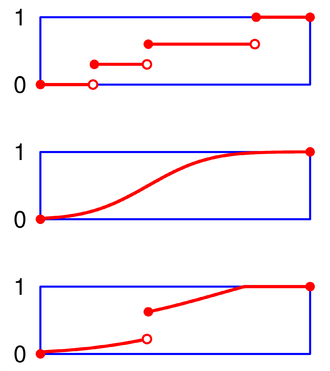
\includegraphics[height = 0.3\textheight]{figures/fonction_repartition}
\caption{\label{fig:fonc:rep} Exemples de fonction de répartition pour une variable aléatoire discrète (haut), continue (centre) ou avec atome (bas). Source \textit{Wikipedia}.}
\end{figure}

Une fonction importante définie à partir de la fonction de répartition est son inverse généralisée. 
Cette fonction est l'outil de la base de la méthode d'inversion décrite plus bas.

\begin{definition}{\textit{Inverse généralisée}}
Soit $F$ une fonction de répartition, on appelle inverse généralisée de $F$, notée, $F^{-1}$ la fonction:
\begin{align*}
\begin{array}{ccl}
]0, 1[&\mapsto& \R\\
u &\mapsto& F^{-1}(u) = \inf\left\lbrace z \in \R \text{ tel que } F(z) \geq u \right\rbrace
\end{array}
\end{align*}
Pour une variable aléatoire $X$, la fonction $F_X^{-1}$ est également appelée \textit{fonction quantile} de la variable aléatoire $X$.
Dans ce cas, on convient que $F_X^{-1}(0)$ et $F_X^{-1}(1)$ sont  la plus petite et la plus grande des valeurs possibles pour $X$ (éventuellement infinies).
\end{definition}

\vspace{\baselineskip}
\textbf{Remarque:} Dans le cas d'une fonction de répartition $F$ continue et strictement croissante sur $\R$\footnote{Associée à une variable aléatoire continue sur $\R$, par exemple}, la fonction $F^{-1}$ est simplement l'inverse de $F$.

\begin{definition}{\textit{Fonction de répartition empirique}}

Soit $X_1, \dots, X_n$ un échantillon de variables aléatoires indépendantes et identiquement distribuées selon la loi d'une variable aléatoire $X$.

La fonction de répartition empirique de la variable aléatoire $X$ associée à $X_1,\dots X_n$, notée $F_X^n$ est la fonction:
\[
\begin{array}{ccl}
\R &\mapsto& [0, 1]\\
x &\mapsto& F_X^n(x) = \frac{1}{n}\underset{i=1}{\overset{n}{\sum}} \mathbf{1}_{X_i \leq x}
\end{array}
\]
On vérifie facilement que $F^n_X$ est une fonction de répartition.
\end{definition}


\subsubsection{Méthode d'inversion}

Supposons qu'on connaisse la fonction de répartition de $X$, $F_X$, alors on a la propriété suivante (propriété d'inversion):

\begin{propriete}{\textit{Méthode d'inversion}}\label{prop:meth:inv}

Soit $F$ une fonction de répartition. Soit $F^{-1}$ son inverse généralisée. Soit $U$ une variable aléatoire de loi uniforme sur $[0, 1]$, alors la variable aléatoire $$X := F^{-1}(U)$$ admet $F$ comme fonction de répartition.
\end{propriete}

\begin{proof}
On veut montrer que, pour tout $x\in \R$ 
\begin{align*}
\mathbb{P}(F^{-1}(U) \leq x) &= F(x).
\intertext{Montrons tout d'abord que, pour tout $u \in ]0, 1[$}
\forall x \in \R,F^{-1}(u) \leq x &\Leftrightarrow u \leq F(x).
\end{align*}
\begin{itemize}
\item[$\Rightarrow$] Soient $u \in ]0, 1[$ et $x\in \R$ tels que $F^{-1}(u) \leq x$. \newline
Par croissance de $F$, on a donc:
\begin{align*}
F\left(F^{-1}(u)\right) &\leq F(x)
\intertext{Or, en se souvenant que par définition}
F^{-1}(u) &= \inf\left\lbrace z \in \R \text{ tel que } F(z) \geq u \right\rbrace,
\intertext{on a donc directement}
u&\leq  F\left(F^{-1}(u)\right) \leq F(x)
\end{align*}
\item[$\Leftarrow$] Soient $u \in ]0, 1[$ et $x\in \R$ tels que $u \leq F(x)$.\newline
Ainsi, $x\in\left\lbrace z \in \R \text{ tel que } F(z) \geq u \right\rbrace$, donc $F^{-1}(u) \leq x$.
\end{itemize}
On a donc montré, l'équivalence. 
Il reste à conclure en se servant de la définition d'une loi uniforme:
$$\mathbb{P}(F^{-1}(U) \leq x) = \mathbb{P}(U \leq F(x))  = F(x).$$
\end{proof}

\textbf{Conséquence et intérêt de la Proposition \ref{prop:meth:inv}:} Comme conséquence immédiate de cette proposition, on obtient une méthode de simulation d'un échantillon pour une variable aléatoire $X$ de loi de probabilité $F_X$:
\begin{enumerate}
\item Calculer $F^{-1}_X$
\item Simuler un échantillon aléatoire i.i.d. $U_1,\dots,U_n$de loi $\Unif[0,1]$\footnote{Qu'on est capable de simuler grâce à un algorithme similaire à ceux décrit en \ref{sec:gen:unif}.}
\item Obtenir un échantillon i.i.d. $X_1,\dots,X_n = F_X^{-1}(U_1),\dots, F_X^{-1}(U_n)$
\end{enumerate} 

\subsubsection{Méthode d'acceptation rejet}

La méthode d'acceptation rejet permet de simuler selon une densité $f$, évaluable en tout point, même lorsque la méthode d'inversion ne peut être appliquée.

L'idée est de se servir d'une loi qu'on sait simuler (la loi de proposition), de densité $g$, et ayant un support couvrant celui de $f$.

\begin{propriete}{\textit{Méthode d'acceptation-rejet}}\label{prop:meth:ar}
Soit $f$ et $g$ deux densités sur $\R^d$.
On suppose qu'il existe une constante $M$ telle que 
$$\forall x \in \R~~f(x) \leq M(g(x))$$
On note 
$$\alpha(x) := \frac{f(x)}{Mg(x)}.$$
Soit $(U_n)_{n\geq 1}$ une suite de variables aléatoires i.i.d. de loi uniforme sur $[0, 1]$. Soit $(Y_n)_{n\geq 1}$ une suite de variables aléatoires i.i.d. de densité $g$.
On note $T$ la variable aléatoire (à valeurs dans $\mathbb{N}^*$):
$$T = \inf\left\lbrace n, \text{ tel que } U_n \leq \alpha(Y_n)\right\rbrace.$$.
Alors, la variable aléatoire $X := Y_T$ ($T$-ième valeur de la suite  $(Y_n)_{n\geq 1}$ a pour densité $f$).
\end{propriete}

\begin{proof}
Soit un entier $n\leq 1$:
\begin{align*}
\mathbb{P}\left(X\leq x, T = n \right) &=  \mathbb{P}\left( U_1 > \alpha(Y_1), \dots, U_{n - 1} > \alpha(Y_{n-1}), U_n \leq \alpha(Y_n), Y_n \leq x  \right)
\intertext{Par propriété d'indépendance}
&= \mathbb{P}\left(U_n \leq \alpha(Y_n), Y_n \leq x  \right)\prod_{i = 1}^{n-1}\mathbb{P}\left(U_i > \alpha(Y_i)\right)
\intertext{Par propriété de distribution identique}
&= \mathbb{P}\left(U_n \leq \alpha(Y_n), Y_n \leq x  \right)\mathbb{P}\left(U_1 > \alpha(Y_1)\right)^{n-1}
%%%%%% PREMIER TERME%%%%
\intertext{Or on a:}
\mathbb{P}\left(U_1 > \alpha(Y_1)\right) &= \E\left[\mathbf{1}_{U_1 > \alpha(Y_1)}\right]\\
&= \int_{\R} \left(\int_0^1 \mathbf{1}_{u > \frac{f(y)}{Mg(y)}} \rmd  u\right)\times g(y) \rmd y\\
&=\int_{\R} (1 -  \frac{f(y)}{Mg(y)})g(y) \rmd y
\intertext{Comme $f$ et $g$ sont des densités:}
\mathbb{P}\left(U_1 > \alpha(Y_1)\right) &=1 - \frac{1}{M}
\intertext{De manière analogue}
\mathbb{P}\left(U_n \leq \alpha(Y_n), Y_n \leq x  \right) &= \E\left[\mathbf{1}_{U_n \leq \alpha(Y_n)}\times \mathbf{1}_{Y_n \leq x}\right]\\
&=  \int_{\R} \left(\int_0^1 \mathbf{1}_{u \leq \frac{f(y)}{Mg(y)}} \rmd  u\right)\times \mathbf{1}_{y \leq x} g(y) \rmd y\\
&= \int_{-\infty}^x \frac{f(y)}{M}\rmd y\\
&= \frac{F(x)}{M},
\intertext{où $F(x)$ est la fonction de répartition associée à $f$. En résumé:}
\mathbb{P}\left(X\leq x, T = n \right) &= \frac{F(x)}{M}\left(1 - \frac{1}{M}\right)^{n - 1}
\end{align*}
Donc on conclut en remarquant que  
$$\mathbb{P}(X\leq x) = \sum_{n = 1}^\infty \mathbb{P}\left(X\leq x, T = n \right) = F(x)$$
\end{proof}

\vspace{\baselineskip}
\textbf{Remarque sur la loi du temps d'attente:} De la preuve, on peut déduire que 
$$\mathbb{P}\left(T = n \right) = \lim_{x \rightarrow \infty}\mathbb{P}\left(X\leq x, T = n \right) = \lim_{x \rightarrow \infty} \frac{F(x)}{M}\left(1 - \frac{1}{M}\right)^{n - 1} =  \frac{1}{M}\left(1 - \frac{1}{M}\right)^{n - 1}$$
Donc, la loi du temps d'attente avant d'obtenir une réalisation de $F$ est une loi géométrique de paramètre $\frac{1}{M}$. 

L'espérance du nombre d'essais avant le premier succès est donc $M$. 

Pour un $g$ donné, l'algorithme est optimal en complexité quand $M$ est minimal.

\vspace{\baselineskip}
\textbf{Cas de lois discrètes} La proposition \ref{prop:meth:ar:disc} permet de simuler pour des variables aléatoires à densité. Un analogue existe pour les variables aléatoires discrètes.

\begin{propriete}{\textit{Méthode d'acceptation-rejet, cas discret}}\label{prop:meth:ar:disc}
Soit $X$ une variable aléatoire discrète sur l'ensemble $\left\lbrace 1,\dots, K\right\rbrace$ et $Y$ une variable aléatoire discrète sur l'ensemble $\left\lbrace 1,\dots, K'\right\rbrace$ (avec $K' \geq K$).
On suppose qu'il existe une constante $M$ telle que 
$$\forall k \in \left\lbrace 1,\dots, K'\right\rbrace~~\mathbb{P}(X = k) \leq M\mathbb{P}(Y=k)$$
On note 
$$\alpha(k) := \frac{\mathbb{P}(X = k)}{M\mathbb{P}(Y=k)}.$$
Soit $(U_n)_{n\geq 1}$ une suite de variables aléatoires i.i.d. de loi uniforme sur $[0, 1]$. Soit $(Y_n)_{n\geq 1}$ une suite de variables aléatoires i.i.d. de même loi que $Y$.
On note $T$ la variable aléatoire (à valeurs dans $\mathbb{N}^*$):
$$T = \inf\left\lbrace n, \text{ tel que } U_n \leq \alpha(Y_n)\right\rbrace.$$
Alors, la variable aléatoire $Y_T$ ($T$-ième valeur de la suite  $(Y_n)_{n\geq 1}$ a la même loi que $X$.
\end{propriete}

\begin{proof}
La preuve est l'analogue pour les lois discrètes de la précédente.
\end{proof}

\subsubsection{Utilisation de transformation usuelles}

On peut bien évidemment utiliser la théorie des probabilités pour simuler différentes lois, notamment les règles sur la stabilité des lois:

\begin{itemize}
\item Si $c > 0$ et $d\in\mathbb{R}$ $U \sim \Unif[a, b] \Rightarrow cU + d \sim \Unif[ac + d, bc + d]$
\item Si $X\sim\Nor (\mu, \sigma^2) \Rightarrow aX +b \sim \Nor(a\mu + b, a^2\sigma^2)$
\item Etc...
\end{itemize}

\subsection{Vecteurs aléatoires}

Supposons qu'on veuille simuler un vecteur aléatoire (X, Y) où $X$ et $Y$ sont deux variables aléatoires réelles (cela s'étend évidemment à un vecteur de taille $n$). 

Un cas simple est quand $X$ et $Y$ sont indépendantes, alors, on se ramène au cas univarié, et le couple aléatoire est donné par deux réalisations indépendantes.

Dans les autres cas, certaines méthodes peuvent s'avérer utiles.

\subsubsection{Conditionnement}

Un cas utile en pratique est le cas où l'on sait simuler facilement $X$, et l'on sait facilement simuler $Y$ sachant $X$. 

On utilise alors la décomposition de la loi jointe

$$\Pro(X\leq x, Y\leq y) = \Pro(Y\leq y \vert X\leq x) \times \Pro(X\leq x)$$

\textbf{Exemple} Supposons qu'on veuille simuler selon la densité jointe:
$$f_{X,Y}(x, y) = x\e{-xy}\I{0\leq x\leq 1}\I{y>0}$$
Alors, la densité marginale de $X$ est donnée par:
$$f_X(x) = \int_0^\infty x\e{-xy}\I{0\leq x\leq 1}\rmd y = \I{0\leq x\leq 1}$$
Ainsi, $X$ suit une loi uniforme sur $[0, 1]$. $x$ étant fixé, la loi de $Y\vert X$ est donnée par une loi exponentielle de paramètre $x$. On peut donc facilement simuler $(X, Y)$ en simulant selon une uniforme, puis une exponentielle de paramètre donné par cette uniforme.

\subsubsection{Changement de variables}

Pour les couples de variables aléatoires à densité, on peut utiliser la propriété du changement de variables. 
\begin{propriete}
Soit un couple de variables aléatoires $(U,V)$ de densité $f_{U,V}(u,v)$ définie sur $E_{UV} \subset \R^2$ et un couple de variables aléatoires $(X, Y)$ à valeurs dans $E_{XY} \subset \R^2$. Supposons qu'il existe une application $\phi$, $C^1$, inversible, et d'inverse $C_1$, tel que $(X, Y) = \phi(U, V)$, alors la densité jointe de $(X, Y)$ est donnée par:
$$f_{X,Y}(x, y) = f_{U,V}(\phi^{-1}(x, y))\vert\det J_{\phi^{-1}}(x, y)\vert  $$
\end{propriete}
où $J_\phi$ désigne la matrice jacobienne d'une application $\phi(u, v)$:
$$J_\phi(u, v) = \begin{pmatrix}
\frac{\delta \phi_1}{\delta u}(u, v) & \frac{\delta \phi_1}{\delta v}(u, v)\\
\frac{\delta \phi_2}{\delta u}(u, v) & \frac{\delta \phi_2}{\delta v}(u, v)
\end{pmatrix}$$

\subsubsection{Simulation d'un vecteur Gaussien}
En pratique, un type de vecteur aléatoire important est le vecteur Gaussien.
En dimension $d$, un vecteur Gaussien $X = \left(X_1,\dots,X_d\right)'$ est un vecteur dont toutes les combinaisons linéaires des composantes sont des lois Gaussiennes sur $\R$.

Il est entièrement caractérisé par le vecteur $\E[X] = \left(E[X_1], \dots, \E[X_d]\right)'$ et sa matrice de variance (covariance) $\Sigma$:
$$\Sigma_{i,j} = \Cov[X_i, X_j]$$
Il se trouve qu'un vecteur Gaussien est stable par transformation affine.

Ainsi, si $X$ est un vecteur Gaussien de paramètres $\mu := \E[X]$ et de variance $\Sigma$, alors pour un vecteur $b$ de taille $d$ et une matrice $d \times d$, alors $$AX + b \sim \Nor(A\mu + b, A\Sigma A').$$
Cette propriété implique qu'on peut simuler tout vecteur Gaussien à partir de $d$ variables aléatoires Gaussiennes indépendantes centrées et réduites. 
Pour une matrice de variance $\Sigma$ voulu, il suffit de trouver $R$ tel que $RR' = \Sigma$. Ce calcul est toujours possible car $\Sigma$ est une matrice semi-définie positive. 

\subsection{Complément: Test statistique d'adéquation à une loi}
\label{sec:test:adequation}

Dans ce chapitre, nous avons défini des algorithmes de simulation  d'échantillons aléatoires. 

Correctement évaluer si un algorithme reproduit un comportement aléatoire est un sujet très vaste en informatique, qui ne sera pas abordé ici (encore une fois, voir \cite{knuth1997art}, ou encore, \citep{cover2006elements}, chapitre 7 sur la théorie de la complexité).

D'un point de vue statistique, la question d'évaluer si un échantillon observé est la réalisation d'un échantillon aléatoire de loi connue est également un problème d'intérêt.

Ce problème peut être traité par différents tests statistiques.
Nous en présenterons ici 2: 
\begin{itemize}
\item Le test du $\chi^2$ d'adéquation (pour l'adéquation a une loi discrète); 
\item Le test de Kolmogorov-Smirnoff, pour l'adéquation a une loi continue
\end{itemize}

\subsubsection{Test du $\chi^2$ d'adéquation}

Le test du $\chi^2$ d'adéquation à une loi permet de tester si un échantillon i.i.d. de v.a. discrètes $X_1,\dots, X_n$, à valeurs dans l'ensemble $\lbrace 1,\dots, K\rbrace$ est distribuée selon une loi multinomiale de paramètre $p^* = (p_1,\dots ,p_K)$.

On définit $N_k = \sum_{i = 1}^n \mathbf{1}_{X_i = k}$ et la variable aléatoire
$$T_n = \sum_{k = 1}^K\frac{(N_k - np_k)^2}{np_k}$$
\paragraph{Propriété: }Quand $n\mapsto \infty$, $T_n$ converge en loi vers un $\chi^2(K - 1)$.
\medskip

Pour le test:
\begin{itemize}
\item[$H_0$] La loi de $X_1$ est $p^*$;
\item[$H_1$] La loi de $X_1$ n'est pas $p^*$,
\end{itemize}
On utilisera $T_n$ comme statistique de test.

Pour un risque de première espèce $\alpha \in ]0, 1[$, 
on aura alors la procédure de test suivante, 

Pour un échantillon observé $x_1,\dots, x_n$, on définit $n_k =  \sum_{i = 1}^n \mathbf{1}_{x_i = k}$. On calcule 
$t_n = \sum_{k = 1}^K\frac{(n_k - np_k)^2}{np_k}$
On rejette alors $H_0$ au risque $\alpha$ si $t_n > z_{1 - \alpha}$ ou $z_{1 - \alpha}$ est le quantile d'ordre 1 - $\alpha$ d'une loi du $\chi^2(n-1)$. 


\subsubsection{Test de Kolmogorov-Smirnoff}

Le test de Kolmogorov-Smirnoff permet de tester l'adéquation échantillon i.i.d. de v.a. continues $X_1,\dots, X_n$ à une loi continue de fonction de répartition $F^*$.

On définit la variable aléatoire
$$T_n = \sqrt{n} \max_{i = 1\dots, n} \vert F_n(X_i) - F(X_i)\vert$$

\textbf{Propriété: }Quand $n\mapsto \infty$, $T_n$ converge en loi vers la variable aléatoire $T$ de fonction de répartition $F_T:$
$$F_T(x) = \left\lbrace 
\begin{array}{lr}
0 & \text{ si } x\leq 0\\
1 - 2 \sum_{k = 1} (-1)^{k + 1} \exp\left(-2 k^2 x^2 \right)& \text{ sinon}
\end{array}
\right.$$
Cette loi est appelée loi de Kolmogorov Smirnoff.


Pour un risque de première espèce $\alpha \in ]0, 1[$, 
on aura alors la procédure de test suivante, 

Pour le test:
\begin{itemize}
\item[$H_0$] La loi de $X_1$ est $F^*$;
\item[$H_1$] La loi de $X_1$ n'est pas $F^*$,
\end{itemize}
On utilisera $T_n$ comme statistique de test.

Pour un échantillon observé $x_1,\dots, x_n$, on calcule la fonction de répartition empirique associée $F_n$ et le $t_n$ correspondant.

On rejette alors $H_0$ au risque $\alpha$ si $1 - F_T(t_n) > 1- \alpha$
\medskip

Ces deux tests peuvent être utiles pour vérifier qu'une méthode de simulation fonctionne.

Nous allons maintenant nous intéresser aux méthodes de simulation proprement dites.


\newpage

\hypertarget{infuxe9rence-bayuxe9sienne}{%
\section{Inférence bayésienne}\label{infuxe9rence-bayuxe9sienne}}

\hypertarget{rappel-sur-le-maximum-de-vraisemblance}{%
\subsection{Rappel sur le maximum de
vraisemblance}\label{rappel-sur-le-maximum-de-vraisemblance}}

En statistique paramétrique, on suppose qu'un ensemble d'observations
\(\mathbf{X}\) est la réalisation d'une variable aléatoire dont la loi
dépend d'un ensemble de paramètres \(\theta\) inconnu et à valeurs dans
un espace \(\Theta\). L'inférence statistique consiste en la définition
d'un estimateur de \(\theta\).

Un estimateur générique commun est l'estimateur du maximum de
vraisemblance.

Le modèle statistique posé permettant d'écrire la loi de \(\mathbf{X}\)
quand on connaît \(\theta\), que l'on note \(L(\mathbf{X}, \theta)\). On
choisit comme estimateur le paramètre \(\hat{\theta}\)
\textit{le plus vraisemblable}, c'est à dire celui qui maximise (en
\(\theta\)) la fonction \(L(\mathbf{X}, \theta)\).

L'estimateur du maximum de vraisemblance pour \(\mathbf{X}\) est donné
par
\(\hat{\theta} = \text{argmax}_{\theta}L(\theta\vert \mathbf{X}) = \frac{\sum_{i=1}^n X_i}{n}\).

Cet estimateur \textbf{est une variable aléatoire}. Sa loi dépend du
modèle, mais asymptotiquement, un thérème central limite nous assure que
sa distribution devient celle d'une loi Normale (dont l'expression de la
variance est connue, au moins en théorie).

Dans ce contexte, le paramètre \(\theta\) est donc une quantité fixe
inconnue. Toute la connaissance sur sa valeur vient des données.

\hypertarget{infuxe9rence-bayuxe9sienne-1}{%
\subsection{Inférence bayésienne}\label{infuxe9rence-bayuxe9sienne-1}}

\hypertarget{connaissance-a-priori-et-duxe9finition-du-posterior}{%
\subsubsection{Connaissance a priori et définition du
posterior}\label{connaissance-a-priori-et-duxe9finition-du-posterior}}

Dans le contexte de l'inférence bayésienne, on supposera que le
paramètre \(\theta\) est lui même aléatoire. On modélisera alors sa loi
sous la forme d'une distribution. Cette distribution est indépendante
des données et s'appelle la distribution \textit{a priori}. Elle reflète
la connaissance (et l'incertitude) que l'on a sur le paramètre. La loi a
priori sur \(\theta\) sera notée \(\pi(\theta)\).

L'objectif de l'inférence bayésienne est d'actualiser cette connaissance
(et son incertitude) grâce au données. La quantité d'intérêt, dans ce
contexte est alors la loi de \(\theta\vert \mathbf{X}\), quand appelle
loi a posteriori (ou posterior). Cette quantité sera notée
\(\pi(\theta \vert \mathbf{X})\).

La formule de Bayes sur le conditionnement permet de lier cette loi a
posteriori à la loi a priori et à la vraisemblance du modèle:

\[\pi(\theta\vert \mathbf{X}) = \frac{\pi(\theta)L(\mathbf{X}\vert \theta)}{\int_\Theta \pi(u)L(\mathbf{X}\vert u)} d u\]

On remarque que le dénominateur ne dépend pas de \(\theta\), il s'agit
d'une constante de normalisation. On écrira souvent cette relation
\[\pi(\theta \vert X) \propto \pi(\theta)L(\mathbf{X}\vert \theta)\] Ce
sont les caractéristiques de cette loi (ses quantiles, ses moments) que
l'on cible dans le contexte de l'inférence bayésienne.

\textbf{L'objectif de l'inférence bayésienne est donc la détermination
de \(\pi(\theta\vert \mathbf{X})\)}.

\hypertarget{choix-du-prior}{%
\subsubsection{Choix du prior}\label{choix-du-prior}}

Pour un nombre de données limité, la \textbf{forme du prior} a un impact
sur la forme du posterior.

La forme du prior peut être choisie en fonction du \emph{savoir expert}
(littérature existante, expériences passées).

\textbf{ATTENTION:} Le support du posterior sera toujours inclu dans le
support du prior.

Si le prior charge tout le support de manière égale, on dit qu'il est
\textbf{non informatif}.

\hypertarget{prior-impropre}{%
\subsubsection{Prior impropre}\label{prior-impropre}}

Si le support de \(\theta\) est sur \(\mathbb{R}\), un prior non
informatif est une ``uniforme sur \(\mathbb{R}\)''. Ceci n'est pas
cependant pas une loi de probabilité!

On peut cependant noter abusivement \(\pi(\theta) \propto 1\). Dans ce
cas, si
\(\frac{L(\mathbf{X}) \vert \theta)}{\int_\Theta L\left(\mathbf{X} \vert \theta\right)\text{d} \theta}\)
définit une loi de probabilité en \(\theta\), alors le posterior
\(\pi(\theta\vert \mathbf{X})\) est bien défini. Le prior est alors dit
\textbf{impropre}.

\hypertarget{estimateurs-bayuxe9siens}{%
\subsubsection{Estimateurs bayésiens}\label{estimateurs-bayuxe9siens}}

Les estimateurs bayésiens sont des quantités liées à la loi à
posteriori.

On mentionnera:

\begin{itemize}
\tightlist
\item
  Le maximum a posteriori (MAP), correspondant à à la valeur de
  \(\theta\) maximisant \(\pi(\theta\vert \mathbf{X})\).
\item
  L'espérance a posteriori
  \[\mathbb{E}[\theta \vert \mathbf{X}] = \int_\theta \pi(\theta \vert \mathbf{X}) \theta d \theta.\]
\item
  Intervalles de crédibilités: Pour toute région
  \(\mathcal{R} \subset \Theta\), on peut quantifier:
  \[\mathbb{P}(\theta \in \mathcal{R} \vert  \mathbf{X}) = \int_\mathcal{R} \pi(\theta \vert \mathbf{X}) \text{d}\theta\]
  Pour \(\alpha \in ]0, 1[\), une région de crédibilité de niveau
  \(1-\alpha\) est une région \(\mathcal{R} \subset \Theta\) telle que
  \[\mathbb{P}(\theta \in \mathcal{R} \vert  \mathbf{X} = \mathbf{x}) = 1 - \alpha\]
  Cet intervalle n'est pas asymptotique, mais \textbf{dépend du prior}.
\end{itemize}

\hypertarget{duxe9termination-du-posterior}{%
\subsubsection{Détermination du
posterior}\label{duxe9termination-du-posterior}}

Il existe deux cas différents en inférence bayésienne:

\begin{itemize}
\tightlist
\item
  Soit la loi a posteriori est dans une famille connue (loi normale, loi
  beta, etc,\ldots{}), alors l'inférence est directe, et tous les
  estimateurs bayésiens peuvent être obtenus facilement.
\item
  Soit la loi a posteriori n'appartient pas à une famille de loi connue.
  Dans ce cas, il faudra obtenir les quantités d'intérêt par méthode de
  Monte Carlo. Pour cela, il faudra souvent être capable d'obtenir un
  échantillon i.i.d. selon la loi a posteriori. Les méthodes vues
  jusqu'alors pourront être utilisées. On verra qu'elles ne suffiront
  pas toujours, et que d'autres méthodes, les méthodes de Monte Carlo
  par chaîne de Markov, aideront à s'en sortir.
\end{itemize}

Une manière astucieuse de se retrouver dans le cas 1 est d'utiliser les
propriétés de conjugaisons de certaines lois. On parlera alors de priors
conjugués au modèle.

Les deux sections suivantes décrivent chacune un exemple illustratif de
ces cas.

\hypertarget{cas-conjuguuxe9-moduxe8le-beta-binomial}{%
\subsection{Cas conjugué: modèle
beta-binomial}\label{cas-conjuguuxe9-moduxe8le-beta-binomial}}

\hypertarget{expuxe9rience-et-question}{%
\subsubsection{Expérience et question}\label{expuxe9rience-et-question}}

On suppose qu'on dispose d'une pièce, et l'on souhaite déterminée si
elle est équilibrée. Pour cela, on effectue \(n\) tirages indépendant de
pile ou face.

\hypertarget{moduxe9lisation}{%
\subsubsection{Modélisation}\label{moduxe9lisation}}

On note \(\mathbf{x} = (x_1, \dots, x_n)\) le résultat du lancer (0 si
\emph{face}, 1 si \emph{pile}). On suppose que ces nombres sont les
réalisations d'un vecteur aléatoire \(\mathbf{X} = (X_1,\dots,X_{n})\)
où les \(X_1, \dots, X_n\) sont indépendantes et identiquements
distribuées de loi \(\mathcal{B}ern(\theta)\) où \(\theta \in ]0, 1[\)
est la probabilité d'obtenir pile.

Donc, la loi jointe de \(\mathbf{X} = (X_1,\dots,X_{n})\) (donc la
vraisemblance pour \(\theta\)) est donnée par:
\[L(\mathbf{X}\vert \theta) = \prod_{k = 1}^{n}\mathbb{P}_\theta(X = X_k) = \theta^{\sum_{k=1}^n X_k}\left(1 - \theta \right)^{n - \sum_{k=1}^n X_k}\]
où \(X \sim \mathcal{B}ern(\theta)\).

\hypertarget{prior}{%
\subsubsection{Prior}\label{prior}}

Pour l'inférence bayésienne, on pose comme \emph{a priori} que
\(\theta \sim \mathcal{B}eta(a, b)\). Cette loi est censée illustrée
notre connaissance indépendante des données sur \(\theta\). Le premier
point trivial est que l'on sait que \(\theta\) est entre 0 et 1, donc on
a choisi une loi ayant ce support.

Ensuite, le choix des paramètres \(a\) et \(b\) déterminera notre a
priori sur al pièce:

\begin{itemize}
\tightlist
\item
  Le cas \(a = b = 1\), correspond à une loi uniforme. Cela traduira un
  a priori non informatif sur \(\theta\), chaque valeur entre \(]0,1[\)
  nous semble également vraisemblable.
\item
  Le cas \(a = b\) avec des valeurs supérieures à 1 traduira un a priori
  où la pièce est équilibrée. De grandes valeurs de \(a\) et \(b\)
  traduiront une plus grande certitude.
\item
  Le cas \(a > b\), traduira un a priori où la pièce est déséquilibrée
  en faveur de pile.
\item
  Le cas \(a < b\), traduira un a priori où la pièce est déséquilibrée
  en faveur de face.
\end{itemize}

La figure ci dessous illustre ces différents a priori:

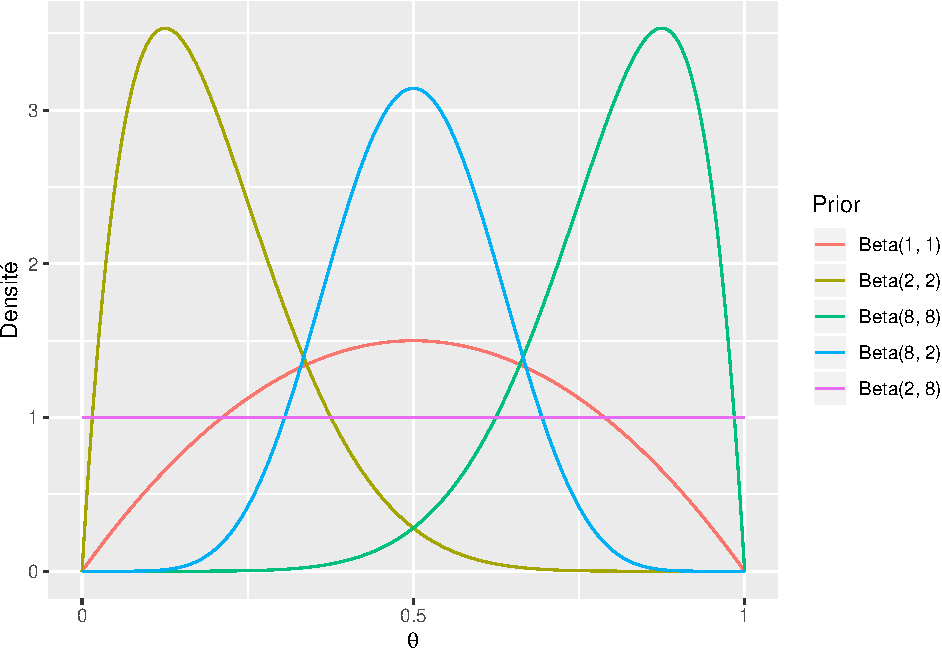
\includegraphics{poly_cours_files/figure-latex/df_prior-1.pdf}

L'expression analytique du prior est donc donnée par:
\[\pi(\theta) = \frac {\theta^{a -1}(1-\theta)^{b -1}}{\int _{0}^{1}u^{a -1}(1-u)^{b -1}\,du}\mathbf{1}_{0 < \theta < 1} \propto \theta^{a -1}(1-\theta)^{b -1}\mathbf{1}_{0 < \theta < 1}\]

\hypertarget{loi-a-posteriori}{%
\subsubsection{Loi a posteriori}\label{loi-a-posteriori}}

On cherche la loi de \(\theta \vert \mathbf{X}\).

On a directement que: \begin{align*}
\pi(\theta \vert\mathbf{X}) &\propto L(\mathbf{X}\vert \theta)\pi(\theta)\\
&\propto \theta^{\sum_{k=1}^n X_k}\left(1 - \theta \right)^{n - \sum_{k=1}^n X_k} \theta^{a -1}(1-\theta)^{b -1}\mathbf{1}_{0 < \theta < 1}\\
&\propto \theta^{a + \sum_{k=1}^n X_k - 1}(1-\theta)^{b + n - \sum_{k=1}^n X_k -1}\mathbf{1}_{0 < \theta < 1}
\end{align*} On reconnaît que \(\pi(\theta\vert \mathbf{X})\) est la
densité d'une loi
\[\theta\vert \mathbf{X} \sim \beta\left(a + \underbrace{\sum_{k = 1}^n X_k}_{\text{Nb. piles}},~b + \underbrace{n - \sum_{k = 1}^n X_k}_{\text{Nb. faces}}\right)\]

Le fait que la \emph{loi a posteriori} soit dans la même famille que la
loi \emph{a priori} est une propriété de conjugaison du modèle binomial
avec le prior de loi beta. Ce prior est dit conjugué.

\hypertarget{estimateurs-bayuxe9siens-1}{%
\subsubsection{Estimateurs bayésiens}\label{estimateurs-bayuxe9siens-1}}

\begin{itemize}
\tightlist
\item
  \textbf{Maximum a posteriori (MAP)}
\end{itemize}

On peut montrer que, pour \(a + b + n > 2\) et
\(a + \sum_{k = 1}^n x_k \geq 1\)
\[MAP(\theta \vert \mathbf{X}) = \frac{a + \sum_{k = 1}^n X_k-1}{a  +  b + n -2}\]
On remarque que pour \(a = b = 1\) (prior uniforme), il s'agit du
maximum de vraisemblance, et que pour tout couple \((a, b)\), cette
quantité converge vers le maximum de vraisemblance quand \(n\) grandit.

\begin{itemize}
\tightlist
\item
  \textbf{Espérance a posteriori}
\end{itemize}

Par propriété de la loi \(\beta\), on:
\[\mathbb{E}[\theta \vert \mathbf{X}] \overset{\text{loi } \beta}{=} \frac{a + \sum_{k = 1}^n X_k}{a + b + n} = \underbrace{\frac{n}{a + b + n}}_{\text{Poids données}}\times \overbrace{\frac{\sum_{k=1}^n X_k}{n}}^{\text{Max. de vrais.}} + \underbrace{\frac{a + b}{a + b + n}}_{\text{Poids prior}} \times \overbrace{\frac{a}{a + b}}^{\mathbb{E}\text{ du prior}}\]

Encore une fois, la décomposition illustre le poids des données et le
poids du prior. On remarque que pour \(n\) suffisament grand, tous les
priors seront équivalents.

\begin{itemize}
\tightlist
\item
  \textbf{Régions de crédibilité}
\end{itemize}

Toute région de crédibilité peut facilement être obtenue à l'aide de la
fonction quantile de la loi \(\beta\), qui est implémentée dans tout
logiciel de statistiques.

\hypertarget{posterior-de-loi-inconnue-moduxe8le-de-ruxe9gression-probit}{%
\subsection{Posterior de loi inconnue: modèle de régression
probit:}\label{posterior-de-loi-inconnue-moduxe8le-de-ruxe9gression-probit}}

\hypertarget{pruxe9diction-de-pruxe9sence-doiseaux}{%
\subsubsection{Prédiction de présence
d'oiseaux}\label{pruxe9diction-de-pruxe9sence-doiseaux}}

Une étude consiste en l'observation de la présence ou non de la linotte
mélodieuse sur différents sites échantillonnés.

Sur ces différents sites sont mesurées différentes caractéristiques:

\begin{itemize}
\tightlist
\item
  Le nombre de vers moyens sur une surface au sol de \(1m^2\).
  (Covariable 1)
\item
  La hauteur d'herbe moyenne sur une surface au sol de \(1m^2\).
  (Covariable 2)
\item
  On calcule cette hauteur d'herbe au carré. (Covariable 3).
\end{itemize}

On peut représenter la présence ou non d'oiseaux en fonctions des
caractéristiques du site:

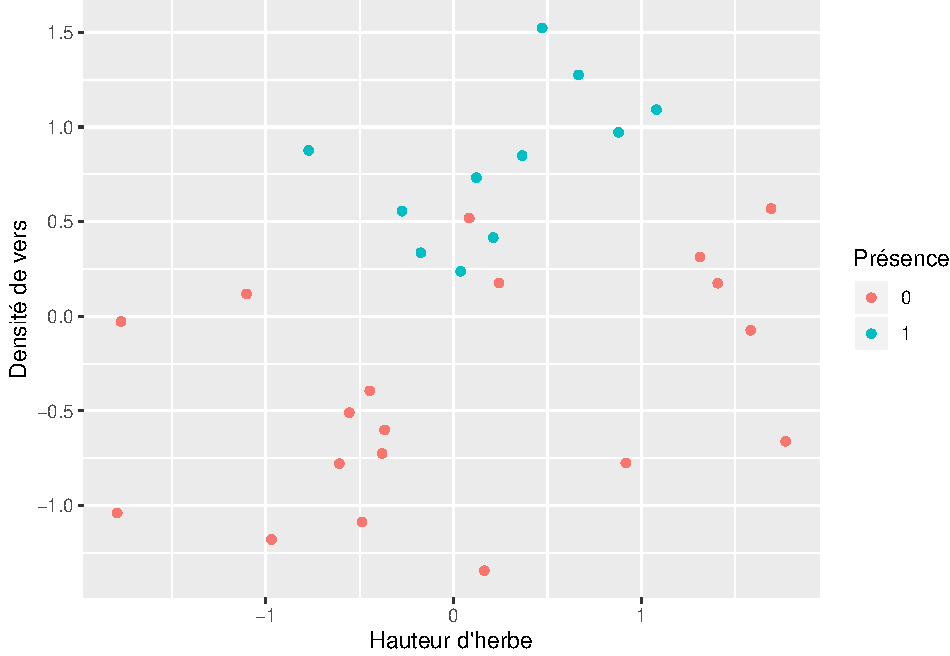
\includegraphics{poly_cours_files/figure-latex/plot_donnees_presence-1.pdf}

\hypertarget{notations-et-moduxe8le-de-ruxe9gression-probit}{%
\subsubsection{Notations et modèle de régression
probit}\label{notations-et-moduxe8le-de-ruxe9gression-probit}}

On note \(y_1, \dots, y_n\) les observations de présence (1 si on
observe un oiseau, 0 sinon) sur les sites \(1\) à \(n\).

On note
\[\mathbf{x}_k = (\overset{\text{Nb. vers}}{x_{k,1}}, \overset{\text{Haut. herbe}}{x_{k,2}}, \overset{\text{Haut. herbe}^2}{x_{k,3}})^T\]
le vecteur des covariables sur le \(k\)-ème site \((1\leq k \leq n)\).

On pose le modèle suivant:

\(Y_k \sim \mathcal{B}ern(p_k)\) où
\[p_k = \phi(\beta_0 + \beta_1 x_{i1} + \beta_2x_{i2} + \beta_3 x_{i3}) = \phi(\mathbf{x}_k^T\theta),\]
où

\begin{itemize}
\tightlist
\item
  \(\phi\) est la fonction de répartition d'une \(\mathcal{N}(0, 1)\),
  i.e.
  \[\phi(z) = \frac{1}{\sqrt{2\pi}}\int_{-\infty}^z \text{e}^{-\frac{u^2}{2}}\text{d}u\]
\item
  \(\theta = \left\lbrace \beta_0, \beta_1, \beta_2, \beta_3\right\rbrace\)
  est le vecteur des paramètres à estimer.
\end{itemize}

\hypertarget{vraisemblance}{%
\subsubsection{Vraisemblance}\label{vraisemblance}}

Pour un vecteur d'observations \(\mathbf{Y} = Y_{1:k}\), la
vraisemblance
\[L(\mathbf{Y}\vert \theta) = \prod_{k = 1}^n \underset{\text{Proba. présence}}{\phi(\mathbf{x}_k^T\theta)^{Y_k}}\times \underset{\text{Proba. absence}}{(1 - \phi(\mathbf{x}_k^T\theta))}^{1 - Y_k}\]

\hypertarget{prior-sur-theta}{%
\subsubsection{\texorpdfstring{Prior sur
\(\theta\)}{Prior sur \textbackslash{}theta}}\label{prior-sur-theta}}

Comme a priori sur \(\theta\), on choisit une normale avec une grande
variance\(\theta \overset{\text{prior}}{\sim} \mathcal{N}(0, 4 I),\)
donc
\[\pi(\theta) = \frac{1}{\sqrt{2\pi \times 4}^4} \text{e}^{-\frac{1}{8}\theta^T\theta}\]
où \(I\) est la matrice Identité (ici \(4 \times 4\))

\hypertarget{posterior}{%
\subsubsection{Posterior}\label{posterior}}

Le posterior est donc donné par:
\[\pi(\theta \vert \mathbf{Y}) \propto \pi(\theta) L(\mathbf{Y}\vert \theta) \propto \frac{1}{64\pi^2}\text{e}^{-\frac{1}{8}\theta^T\theta} \prod_{k = 1}^n \phi(\mathbf{x}_k^T\theta)^{Y_k} (1 - \phi(\mathbf{x}_k^T\theta))^{1 - Y_k}\]

Cette densité n'est pas standard. Ainsi, on ne connaît pas ces
caractéristiques associées et intéressantes (quantiles, espérance,
variance). Ces différentes quantités peuvent cependant être approchées
par méthode de Monte Carlo, si tant est qu'on soit capable de simuler
selon cette loi.

\hypertarget{simulation-duxe9chantillons-a-posteriori-par-acceptation-rejet}{%
\subsubsection{Simulation d'échantillons a posteriori par acceptation
rejet}\label{simulation-duxe9chantillons-a-posteriori-par-acceptation-rejet}}

Notre objectif est de simuler selon le posterior défini ci dessus. On va
pour ce faire procéder par méthode d'acceptation rejet.

On remarque immédiatement qu'on ne peut pas utiliser l'acceptation rejet
classique, car \(\pi(\theta \vert \mathbf{Y})\) n'est connu qu'à une
cnstante près!

Cependant, si on note
\[\tilde{\pi}(\theta \vert \mathbf{Y}) = \frac{1}{64\pi^2}\text{e}^{-\frac{1}{8}\theta^T\theta} \prod_{k = 1}^n \phi(\mathbf{x}_k^T\theta)^{Y_k} (1 - \phi(\mathbf{x}_k^T\theta))^{1 - Y_k},\]
on peut utiliser la propriété vue en TD, qui dit qu'il suffit de
connaître \(\tilde{\pi}\) pour simuler selon \(\pi\) à partir
d'acceptation rejet.

\begin{itemize}
\tightlist
\item
  \textbf{Choix de la densité de proposition}
\end{itemize}

Comme densité de proposition, on peut par exemple prend pour \(g\) la
densité correspondant au prior (\(g(\theta) = \pi(\theta)\)). On
remarque que dans ce cas
\[\frac{\tilde{\pi}(\theta \vert \mathbf{Y})}{g(\theta)} = \frac{\pi(\theta)L(\mathbf{Y}\vert \theta)}{\pi(\theta)} = \prod_{k = 1}^n \phi(\mathbf{x}_k^T\theta)^{Y_k} (1 - \phi(\mathbf{x}_k^T\theta))^{1 - Y_k} \leq 1 =:M.\]

On a donc un majorant uniforme en \(\theta\) et l'acceptation rejet
suivant permet de tirer selon \(\pi(\theta \vert \mathbf{Y})\):

\begin{enumerate}
\def\labelenumi{\arabic{enumi}.}
\tightlist
\item
  On tire \(\theta_{cand} \sim \mathcal{N}(0, 4I)\)
\item
  On tire (independamment) \(U\sim \mathcal{U}[0, 1]\)
\item
  Si \(U < \frac{L(y_{1:n}\vert \theta)}{M}\), on accepte
  \(\theta_{cand}\)
\item
  Sinon on recommence
\end{enumerate}

\hypertarget{echantillon-du-posterior-loi-a-posteriori-marginales-et-estimateurs-bayuxe9siens}{%
\subsubsection{Echantillon du posterior, loi a posteriori marginales et
estimateurs
bayésiens}\label{echantillon-du-posterior-loi-a-posteriori-marginales-et-estimateurs-bayuxe9siens}}

\begin{itemize}
\tightlist
\item
  \textbf{Lois marginales}
\end{itemize}

On effectue un tirage de taille \(M = 1000\). On peut représenter la
densité empirique de cet échantillon

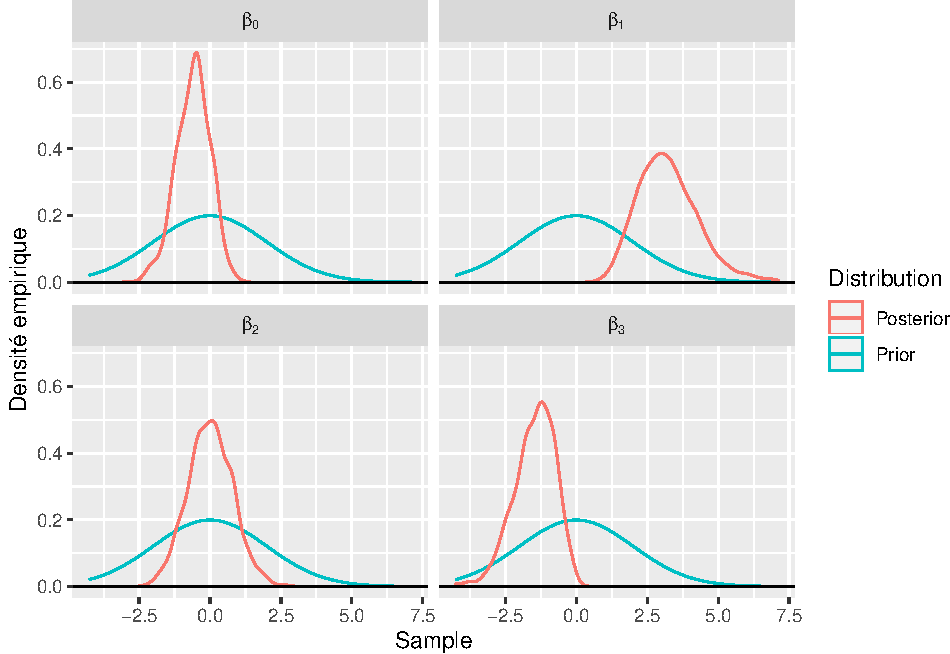
\includegraphics{poly_cours_files/figure-latex/plot_posterior_samples-1.pdf}

On peut remarquer que les densités du posterior sont différentes du
prior.

\begin{itemize}
\tightlist
\item
  \textbf{Loi jointe}
\end{itemize}

Il peut être intéressé de regarder la loi jointe obtenue par simulation.
On pourra notamment remarquer qu'un prior indépendant sur les
composantes n'entraîne pas une indépendance dans le posterior. Par
exemple, on représente ici la loi du couple
\((\beta_0,\beta_1 \vert \mathbf{Y})\):

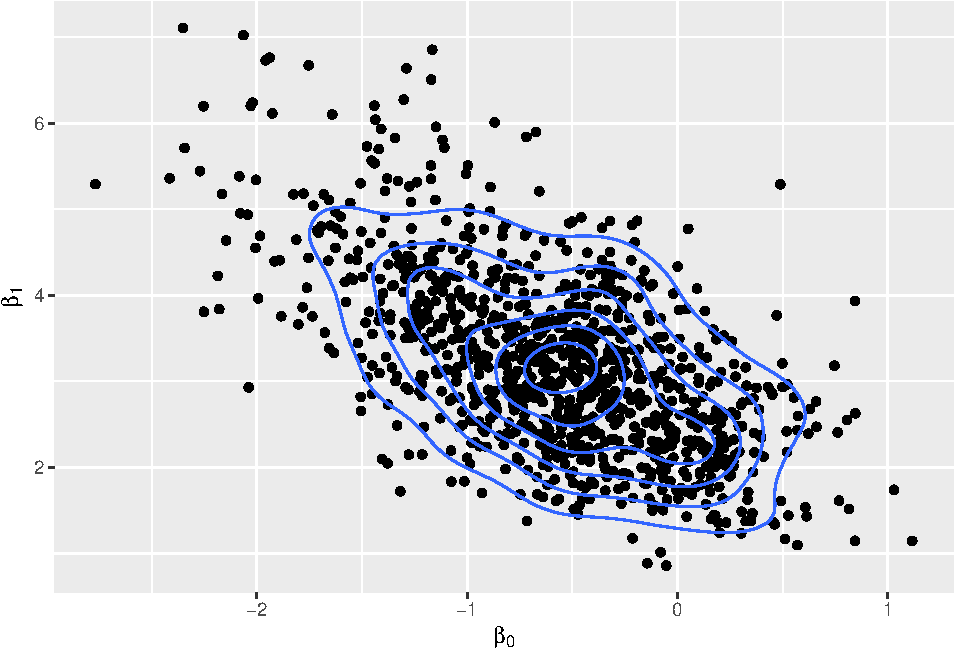
\includegraphics{poly_cours_files/figure-latex/loi_jointe_beta0_beta1-1.pdf}

On voit qu'il existe une correlation linéaire négative entre ces deux
variables aléatoires, qui étaient, a priori, supposées indépendantes.

\begin{itemize}
\tightlist
\item
  \textbf{Espérance a posteriori et intervalles de crédibilité}
\end{itemize}

Comme on sait simuler selon la loi cible, les espérances peuvent être
approchées par méthode de Monte Carlo classique. On obtient ici une
estimation del'espérance \textbf{a posteriori} ainsi qu'un intervalle de
confiance a posterirori

\begin{longtable}[]{@{}lrrr@{}}
\toprule
Paramètre & Esperance a posteriori. & Quantile 2.5\% & Quantile
97.5\%\tabularnewline
\midrule
\endhead
beta{[}0{]} & -0.593 & -1.915919 & 0.5002617\tabularnewline
beta{[}1{]} & 3.228 & 1.485531 & 5.7121958\tabularnewline
beta{[}2{]} & 0.011 & -1.513225 & 1.5548755\tabularnewline
beta{[}3{]} & -1.472 & -3.051512 & -0.2826136\tabularnewline
\bottomrule
\end{longtable}

\hypertarget{au-deluxe0-de-lacceptation-rejet}{%
\subsection{Au delà de l'acceptation
rejet}\label{au-deluxe0-de-lacceptation-rejet}}

Dans le cas précédent, l'espérance du temps d'attente avant une
acceptation est donnée par
\[\frac{M}{\int L(\mathbf{Y}\vert \theta)\pi(\theta) \text{d}\theta}\]

Mécaniquement, cette quantité augmente quand \(n\) augmente, et
l'acceptation rejet dvient prohibitif.

En pratique, l'inférence Bayésienne utilisera d'autres algorithmes de
simulations de loi: les algorithmes de Monte Carlo par chaîne de Markov.

\newpage

\hypertarget{muxe9thodes-de-monte-carlo-par-chauxeene-de-markov}{%
\section{Méthodes de Monte Carlo par chaîne de
Markov}\label{muxe9thodes-de-monte-carlo-par-chauxeene-de-markov}}

Il n'est pas toujours possible de simuler (efficacement) un échantillon i.i.d. selon une densité cible $f$.

Cependant, il existe des outils permettant de construire des chaînes de Markov dont la distribution asymptotique sera donnée par $f$. 
La chaîne de Markov ainsi construite permettra l'approximation d'espérance par rapport à $f$ grâce à une version "Chaîne de Markov" de la loi des grands nombres.

Le but de ce chapitre est de présenter l'algorithme de Metropolis-Hastings, méthode très générique pour construire une chaîne de Markov adaptée. 

Cet algorithme est très générique et est définit aussi bien que pour des lois discrètes, que pour des lois à densité.

On introduira ici l'algorithme (et la preuve de son fonctionnement), dans le cas discret. La cas continu est présenté bien plus rigoureusement dans \citep{robert2013monte}.


\subsection{Rappel sur les chaînes de Markov}
On se place dans un ensemble $\K$ fini (typiquement l'ensemble $\left\lbrace 1,\dots, K\right\rbrace$).

\begin{definition}{\textit{Chaîne de Markov}}
Soit $X_0$ une variable aléatoire sur $\K$ de loi $\pi_0$.
On dit que la suite de variables aléatoires $(X_n)_{n\geq 0}$ à valeurs $\K$ dans est une chaîne de Markov si pour tout $n\geq 1$ est pour tout suite $(k_0,\dots,k_n)$ d'éléments de $\K$, on a :

$$\Pro\left( X_n = k_n \vert X_0 = k_0,\dots,X_{n- 1} = k_{n- 1}\right) = \Pro(X_n = k_n \vert X_{n-1} = k_{n-1})$$
On dit que cette chaîne de Markov est $\textit{homogène}$ si, pour $i$ et $j$ dans $\K$: 
 $\Pro(X_n = j \vert X_{n-1} = i) = \Pro(X_1 = j \vert X_{0} = i) = P_{ij}$
 La matrice $P = (P_{ij})$ est alors appelée matrice de transition de la chaîne de Markov. $P_{ij}$ est la probabilité de transition de $i$ vers $j$. Dans la suite on se placera dans le cas homogène.
 Une chaîne de Markov homogène est entièrement caractérisée par $\pi_0$ et $P$.
 
 On remarque immédiatement que $0 \leq P_{ij}\leq 1 $ et $\sum_{j}P_{ij} = 1$ 
\end{definition}

\paragraph{Propriétés} On rappelle quelques propriétés utiles.
On note $\pi_n$, pour $n \geq 0$ la loi de l'état $X_n$, c'est à dire le vecteur ligne $$\pi_n = (\pi_{n,1} = \Pro(X_n = 1),\dots,\pi_{n, K} = \Pro(X_n = K)).$$
On a alors:

\begin{itemize}
\item $\Pro(X_1 = j) = \sum_{i = 1}^k \Pro(X_0 = i) \times \Pro(X_1 = j \vert X_0 = i) = \sum_{i = 1}^k \pi_{0,i}P_{ij}$ 
Cette relation est résumée par l'équation $\pi_1 = \pi_0P$
\item On peut montrer par récurrence que 
$$P^{(n)}_{ij} := \Pro(X_n = j\vert X_0 = i) = (P^n)_{ij}$$ où $P^n$ est la puissance $n$-ième de la matrice $P$. 
\item On a ainsi: $$\pi_n = \pi_0P^n$$
\end{itemize}

\begin{definition}{\textit{Mesure invariante pour $P$}}
Soit $\pi$ un vecteur (ligne) de probabilité (une mesure de probabilité sur $\K$). On dit que $\pi$ est invariante pour la chaîne de Markov de transition $P$ si:
$$\pi P = \pi$$ 
\end{definition}

Comme conséquence immédiate, on a que si $\pi_0$ est une mesure invariante pour $P$, alors, pour tout $n$, $\pi_n = \pi_0$. Dans ce cas, les variables aléatoires $X_0,\dots, X_n$ sont identiquement distribuées (mais pas indépendantes!).

\begin{definition}{\textit{Irréductibilité de P}}
On dit qu'une chaîne de Markov homogène sur $\K$, de transition $P$ est irréductible si 
$$\forall i,j \in \K\times \K,~\exists~n \text{ tel que } P^{(n)}_{i,j} > 0$$
Autrement dit, pour deux états de la chaîne, il est possible d'accéder de l'un à l'autre en un temps fini. 
\end{definition}

\begin{definition}{Chaîne apériodique}
Soit $(X_n)_{n\geq 1}$ une chaîne de Markov homogène sur $\K$. Pour $k \in \K$, on appelle \textit{période} de l'état $k$, notée $d(k)$, le P.G.C.D. de tous les entiers $n$ tels que $P^{(n)}_{kk} > 0$ (avec la convention $pgcd(\emptyset) = +\infty$):
$$d(j) = pgcd\left\lbrace n\geq 1, P^{(n)}_{kk} > 0\right\rbrace$$
Une chaîne est dite apériodique si pour tout $k$ dans $\K$, $d(k) = 1$.
Pour une chaîne irréductible, une condition suffisante pour être apériodique est qu'il existe un $k\in \K$ tel que $P_{kk} > 0$.
\end{definition}

\begin{propriete}{\textit{Théorème ergodique}}
\label{prop:theo:ergo}
Soit $(X_n)_{n\geq 0}$ une chaîne de Markov de loi initiale $\pi_0$ et de matrice de transition $P$. On suppose que cette chaîne est  irréductible et apériodique.
Alors: 

\begin{enumerate}
\item Cette chaîne de Markov admet une unique mesure de probabilité invariante $\pi$.
\item $X_n \overset{loi}{\longrightarrow} X$ où $X$ est une v.a. de loi $\pi$.
\item Pour toute fonction $\varphi$ intégrable par rapport à $\pi$, on a :
$$\frac{1}{n + 1} \sum_{i = 0}^n \varphi(X_i) \underset{n \rightarrow +\infty}{\overset{p.s.}{\longrightarrow}} \mathbb{E}_\pi[\varphi(X)].$$
\item Si $\varphi(X)$ admet un moment d'ordre supérieur à 2, on a
 $$\sqrt{n}\left( \frac{1}{n + 1}\sum_{i = 0}^n \varphi(X_i) - \mathbb{E}_\pi[\varphi(X)] \right) \underset{n \rightarrow +\infty}{\overset{Loi}{\longrightarrow}} \mathcal{N}(0, \sigma^2)$$
\end{enumerate}
\end{propriete}

Un analogue de cette propriété reste vrai quand la chaîne de Markov est à valeurs dans un ensemble continu (typiquement, $\R^d$). Si le résultat reste moralement le même, il demande un formalisme plus conséquent. On pourra se référer à \citep{robert2013monte} pour une présentation rigoureuse.

\paragraph{Remarque sur le Théorème Central Limite}
Contrairement au TCL dans le cas i.i.d., la variance $\sigma^2$ n'est absolument pas triviale (il ne s'agit pas de $\V[\varphi(X)]$!), et n'est pas nécessairement facile à estimer. En effet, les variables aléatoires dans l'estimateur Monte Carlo ne sont plus indépendantes, on ne peut donc plus considérer la variance de l'estimateur comme la somme des variances. Ainsi, obtenir un estimateur de la variance (et donc un intervalle de confiance asymptotique) n'est pas nécessairement évident.

\paragraph{Conséquence et intérêt pratique de la Proposition \ref{prop:theo:ergo}} Le théorème ergodique pour les chaînes de Markov stipule qu'il n'est pas nécessaire de savoir simuler un échantillon i.i.d. pour obtenir une approximation de l'espérance selon une loi $\pi$ (ou une densité $f$, ce qui nous intéressera plus souvent en pratique). En effet, si l'on est capable de construire une chaîne de Markov irréductible de mesure de probabilité invariante $\pi$ (ou $f$), alors, en simulant selon cette chaîne de Markov suffisamment longtemps, on pourra approcher toute espérance relativement à $\pi$. De plus, le point 2. de la proposition nous assure qu'au bout d'un certain temps, les $X_n$ obtenus pourront être considérés comme de loi $\pi$ (mais pas indépendants!). Encore faut il être capable de construire une chaîne de Markov (une matrice $P$) irréductible, de loi invariante donnée par $\pi$.

C'est le sens de l'algorithme de Metropolis Hastings.

\subsection{Algorithme de Metropolis-Hastings}

\subsubsection{Définitions}

\begin{definition}{\textit{Réversibilité}}
Soit $\pi =(\pi_1,\dots, \pi_K)$ une mesure de probabilité sur $\K$ et $(X_n)_{n\geq 0}$ une chaîne de Markov homogène de matrice de transition $P$. 
On dit que $\pi$ est réversible pour $P$ si elle vérifie la condition d'équilibre:
$$\forall (i, j) \in \K\times \K,~\pi_i \times P_{ij} = \pi_j \times P_{ji}$$
\begin{propriete}{\textit{Réversibilité $\Rightarrow$ Invariance}}
\label{prop:Rev:Inv}
Si une mesure de probabilité $\pi$ est réversible pour une chaîne de Markov de transition $P$, alors, $\pi$ est une mesure de probabilité invariante pour $P$.
\end{propriete}
\begin{proof}
Soit $\pi$ une mesure de probabilité réversible pour $P$. On a tout de suite que
\begin{align*}
\forall j \in \K~~(\pi P)_j & = \sum_{i = 1}^{K} \pi_i P_{ij}& \\
&= \sum_{i = 1}^{K} \pi_j P_{ji} &\text{ par réversibilité}\\
&= \pi_j &\text{ par propriété de } P\\
\Rightarrow \pi P &= \pi&
\end{align*}
\end{proof}
Cette propriété va nous permettre de construire une chaîne de Markov satisfaisant les hypothèses de la Proposition \ref{prop:theo:ergo}.
\end{definition}

\subsubsection{Algorithme dans le cas discret}

\begin{propriete}{\textit{Algorithme de Metropolis Hastings}}
Soit $\pi$ une mesure de probabilité sur $\K$ selon laquelle on aimerait simuler (on supposera que $\pi_k > 0$ pour tout $k$).
Soit $\pi_0$ une mesure de probabilité sur $\K$ telle que $\pi_k > 0\Rightarrow \pi_{0,k} > 0$ et $Q$ une matrice stochastique $\K \times \K$ satisfaisant la condition suivante:
$$\forall (i, j) \in \K\times \K, Q_{ij} > 0 \Leftrightarrow Q_{ji} > 0$$ 

On considère la suite de variables aléatoires $(X_n)_{n\geq 0}$ construite de la manière suivante:
\begin{enumerate}
\item On simule $X_0$ selon $\pi_0$.
\item Pour $n\geq 1$:
\begin{enumerate}
\item On tire $Y_n$ selon la loi $Q_{X_{n-1}\bullet}$ (la ligne de $Q$ donnée par $X_{n-1}$).
\item On tire une loi uniforme $U$ indépendante de $Y_n$.
\item On calcule la quantité 
$$\alpha(X_{n-1}, Y_n) = \min\left(1, \frac{\pi_{Y_n}Q_{Y_n X_{n-1}}}{\pi_{X_{n - 1}}Q_{X_{n-1}Y_n}}\right)$$
\item On pose:
$$X_n = \left\lbrace
\begin{array}{lr}
Y_n & \text{ si } U\leq\alpha(X_{n-1}, Y_n)\\
X_{n - 1} &\text{ sinon}
\end{array}
 \right.$$
\end{enumerate}
\end{enumerate}
alors, $(X_n)_{n \geq 1}$ est une chaîne de Markov de transition $P$ où
$$P_{ij} = \left\lbrace \begin{array}{lr}
Q_{ij}\alpha(i, j) & \text{ si } i\neq j\\
1 - \sum_{j\neq i} P_{ij} &\text{ sinon}
\end{array} \right.$$
De plus $\pi$ est invariante pour $P$.
\end{propriete}
\begin{proof}
La loi de $X_n \vert X_{0:(n-1)}$ ne dépendant que de $X_{n-1}$, la propriété de Markov est évidente par construction. Pour $i\neq j$, on a
\begin{align*}
\Pro(X_{n} = j \vert X_{n -1} = i) &= \Pro\left(Y_{n} = j , U\leq \alpha(X_{n-1}, Y_{n})\vert X_{n -1} = i \right)\\
&=  \Pro\left(Y_{n} = j , U\leq \alpha(i, j)\vert X_{n -1} = i \right)\\
&=\Pro\left(Y_{n} = j \vert X_{n-1} = x\right)\Pro\left( U\leq \alpha(i, j)\vert X_{n -1} = i \right)\\
&= Q_{ij}\alpha(i,j)
\end{align*}
Ce qui prouve la première partie. De plus, pour $i\neq j$, on a:
\begin{align*}
\pi_iP_{ij} &=  \pi_i Q_{ij}\alpha(i, j)\\
&= \pi_i Q_{ij} \min\left(1, \frac{\pi_{j}Q_{j, i}}{\pi_{i}Q_{i,j}}\right)\\
&= \min\left(\pi_i Q_{ij}, \pi_{j}Q_{j, i}\right)\\
&= \pi_{j}Q_{j, i}\min\left(\frac{\pi_i Q_{ij}}{ \pi_{j}Q_{j, i}}, 1 \right)\\
&= \pi_{j}Q_{j, i}\alpha(j,i)\\
&=\pi_{j}P_{j,i}
\end{align*}
Donc, $\pi$ est réversible pour $P$, donc par la proposition \ref{prop:Rev:Inv}, $\pi$ est invariante.
On remarquera que si $Q$ est irréductible et apériodique, $P$ l'est aussi, et ainsi, les conditions de la proposition \ref{prop:theo:ergo} sont satisfaites.
\end{proof}

\subsubsection{Algorithme dans le cas continu}

Supposons qu'on veuille simuler dans $\R^d$ selon une densité $f$, éventuellement connue à une constante près, c'est à dire que 
$$\forall x \in \R^d,~f(x) = C f^{(u)}(x) = \frac{f^{(u)}(x)}{\int_{\R^d}f^{(u)}(z)\rmd z}$$
On remplace alors la matrice de transition par un $\textit{noyau de transition}$ sur $\R^d$, à savoir une fonction
\begin{equation*}
\begin{array}{lccc}
q:& \R^d\times \R^d &\mapsto& \R_+\\
& (x, y) & \mapsto & q(x, y)\geq 0
\end{array}
\end{equation*}
telle que $\int_{\R^d}q(x, y)\rmd y = 1$ (typiquement, la loi d'une marche aléatoire centrée en $x$.

Alors, si on sait simuler, pour $x$ fixé, selon $q$, et qu'on a $q(x, y) > 0 \Leftrightarrow q(y, x) > 0$, alors, l'algorithme de Metropolis reste valide en remplaçant $\pi$ par $f^{(u)}$ et $Q$ par $q$. On notera que dans le ratio on a pas besoin de la constante de normalisation car 
$$\frac{f^{(u)}(y)}{f^{(u)}(x)} = \frac{f(y)}{f(x)}$$

\paragraph{Conséquence et intérêt de l'algorithme de Metropolis Hastings} L'algorithme de Metropolis Hastings est très puissant, car il permet, sous des conditions faibles, de simuler une chaîne de Markov satisfaisant le théorème ergodique. Il s'agit d'un des algorithmes les plus utilisés en pratique. Un de ces défauts est sa nécessité d'avoir une étape d'acceptation rejet. Ainsi, si la probabilité d'acceptation est faible, la chaîne simulée pourra rester "coincée" dans un état, et la variance de l'estimateur Monte Carlo sera très grande.

\subsection{Échantillonneur de Gibbs}

On considère une vecteur aléatoire en dimension $d$ $X = (X^{(1)},\dots, X^{(d)})$.
Dans le cas où la loi $f$ (ou la loi $\pi$) est une densité dans en grande dimension ($\R^d$ ou $\K^d$), l'espace à visiter est typiquement grand, et le ratio d'acceptation de l'algorithme de Metropolis Hastings sera souvent assez faible.

Un algorithme très utilisé dans ce cas est l'échantillonneur de Gibbs.

Cet algorithme suppose que l'on sait simuler  selon \textbf{toutes les lois conditionnelles de $X$}. 

Plus formellement, si on note $X^{-(\ell)} =  (X^{(1)},\dots, X^{(\ell-1)}, X^{(\ell+1)}, X^{(d)})$, on est capable de simuler facilement la variable aléatoire $X^{(\ell)}\vert X^{(-\ell)}$, selon la loi $\pi^{(-\ell)}$. 
Dans ce cas, l'idée est la suivante: 
\begin{enumerate}
\item Prendre $X_0 = (X_0^{(1)},\dots, X_0^{(d)})$ tiré selon une loi initiale.
\item Pour $k \geq 1$:
\begin{enumerate}
\item Tirer $\ell$ uniformément dans $\lbrace1,\dots,d\rbrace$
Actualiser $X_k^{(1)}$ en simulant selon la loi de $X_k^{(1)}\vert X_{k - 1}^{(2)},\dots , X_{k - 1}^{(d)}$;
\item Simuler $Y$ selon la loi $X^{(\ell)} \vert \lbrace X^{(-\ell)} = X_{k-1}^{(-\ell)} \rbrace$
\item Poser $X_k = (X_{k - 1}^{(1)},\dots, X_{k-1}^{(\ell-1)}, Y, X_{k - 1}^{(\ell+1)}, X_{k-1}^{(d)})$
\end{enumerate} 
\end{enumerate}

On peut montrer que l'échantillonneur de Gibbs est équivalent à un algorithme de Metropolis Hastings où la quantité $\alpha$ est toujours égale à 1, c'est à dire un Metropolis Hastings où ne rejette jamais le candidat.

Encore une fois, cet algorithme fonctionne est utile dès que la simulation des lois conditionnelles est faisable. Si les lois conditionnelles induisent une matrice de transition (ou un noyau) de Markov irréductible et apériodique, alors le théorème ergodique s'applique.

\bibliographystyle{abbrv}
\bibliography{references}
\end{document}

\newpage

\bibliographystyle{abbrv}
\bibliography{references}


\end{document}
